\documentclass[a4paper]{article}
\usepackage[spanish]{babel}
\usepackage[utf8]{inputenc}
\usepackage{fancyhdr}
\usepackage{charter} % tipografia
%\usepackage{graphicx}
\usepackage[pdftex]{graphicx}
\usepackage{sidecap}
\usepackage{caption}
\usepackage{subcaption}
\usepackage{booktabs}
\usepackage{makeidx}
\usepackage{float}
\usepackage{amsmath, amsthm, amssymb}
\newtheorem{theorem}{Teorema}[section]
\newtheorem{corollary}{Corolario}[theorem]
\newtheorem{lemma}[theorem]{Lema}
\usepackage{amsfonts}
\usepackage{sectsty}
\usepackage{charter}
\usepackage{wrapfig}
\usepackage{listings}
\usepackage{hyperref} % links
\usepackage{algorithm} %http://www.ctan.org/pkg/algorithms
\usepackage{algorithmic}
\usepackage{color} % para snipets de codigo coloreados
\usepackage{fancybox} % para el sbox de los snipets de codigo
\definecolor{litegrey}{gray}{0.94}
% \newenvironment{sidebar}{%
% \begin{Sbox}\begin{minipage}{.85\textwidth}}%
% {\end{minipage}\end{Sbox}%
% \begin{center}\setlength{\fboxsep}{6pt}%
% \shadowbox{\TheSbox}\end{center}}
% \newenvironment{warning}{%
% \begin{Sbox}\begin{minipage}{.85\textwidth}\sffamily\lite\small\RaggedRight}%
% {\end{minipage}\end{Sbox}%
% \begin{center}\setlength{\fboxsep}{6pt}%
% \colorbox{litegrey}{\TheSbox}\end{center}}

%\newenvironment{codesnippet}{%
%\begin{Sbox}\begin{minipage}{\linewidth-2\fboxsep-2\fboxrule-4pt}\sffamily\small}%
%{\end{minipage}\end{Sbox}%
%\begin{center}%
%\colorbox{litegrey}{\TheSbox}\end{center}}

% \newenvironment{codesnippet}{\VerbatimEnvironment%
%   \noindent
%   %{\columnwidth-\leftmargin-\rightmargin-2\fboxsep-2\fboxrule-4pt}
%   \begin{Sbox}
%   \begin{minipage}{\linewidth-2\fboxsep-2\fboxrule-4pt}
%   \begin{Verbatim}
% }{%
%   \end{Verbatim}
%   \end{minipage}
%   \end{Sbox}%
%   \colorbox{litegrey}{\TheSbox}
% }

\newenvironment{codesnippet}{\VerbatimEnvironment%
  \noindent
  %      {\columnwidth-\leftmargin-\rightmargin-2\fboxsep-2\fboxrule-4pt}
  \begin{Sbox}
  \begin{minipage}{\linewidth}
  \begin{Verbatim}
}{%
  \end{Verbatim}
  \end{minipage}
  \end{Sbox}%
  \colorbox{litegrey}{\TheSbox}
}
\usepackage{fancyhdr}
\pagestyle{fancy}
%\renewcommand{\chaptermark}[1]{\markboth{#1}{}}
\renewcommand{\sectionmark}[1]{\markright{\thesection\ - #1}}
\fancyhf{}
\fancyhead[LO]{Sección \rightmark} % \thesection\
\fancyfoot[LO]{\small{Iv\'an Arcuschin, Mart\'in Jedwabny, Jos\'e Massigoge, Lucas Puterman}}
\fancyfoot[RO]{\thepage}
\renewcommand{\headrulewidth}{0.5pt}
\renewcommand{\footrulewidth}{0.5pt}
\setlength{\hoffset}{-0.8in}
\setlength{\textwidth}{16cm}
%\setlength{\hoffset}{-1.1cm}
%\setlength{\textwidth}{16cm}
\setlength{\headsep}{0.5cm}
\setlength{\textheight}{25cm}
\setlength{\voffset}{-0.7in}
\setlength{\headwidth}{\textwidth}
\setlength{\headheight}{13.1pt}
\renewcommand{\baselinestretch}{1.1} % line spacing
% \setcounter{secnumdepth}{2}
\usepackage{underscore}
\usepackage{caratula}
\usepackage{url}
\usepackage[usenames,dvipsnames]{xcolor}
\lstset{
    language=C++,
    basicstyle=\ttfamily,
    keywordstyle=\color{blue}\ttfamily,
    stringstyle=\color{red}\ttfamily,
    commentstyle=\color{ForestGreen}\ttfamily,
    morecomment=[l][\color{magenta}]{\#}
}

% *********************** %
% Ejercicio 2 - Agregado
% Grafos
\usepackage{tikz}
\usetikzlibrary{graphs}
\usetikzlibrary{calc}
\usetikzlibrary{arrows}
% Otros
\usepackage{arrayjobx}
\usepackage{enumitem}
\usepackage{multicol}
\usepackage{pgfplots}
% *********************** %

% ******************************************************** %
% TEMPLATE DE INFORME ORGA2 v0.1 %
% ******************************************************** %
% ******************************************************** %
% %
% ALGUNOS PAQUETES REQUERIDOS (EN UBUNTU): %
% ========================================
% %
% texlive-latex-base %
% texlive-latex-recommended %
% texlive-fonts-recommended %
% texlive-latex-extra? %
% texlive-lang-spanish (en ubuntu 13.10) %
% ******************************************************** %
\begin{document}
\thispagestyle{empty}
\materia{Algoritmos y Estructura de Datos III}
\submateria{Primer Cuatrimestre de 2015}
\titulo{Trabajo Práctico II}
%\subtitulo{Grupo: }
\integrante{Iv\'an Arcuschin}{678/13}{iarcuschin@gmail.com}
\integrante{Mart\'in Jedwabny}{885/13}{martiniedva@gmail.com}
\integrante{Jos\'e Massigoge}{954/12}{jmmassigoge@gmail.com}
\integrante{Lucas Puterman}{830/13}{lucasputerman@gmail.com}
\maketitle
% no footer on the first page
\thispagestyle{empty}
\newpage

\tableofcontents

\newpage
\section{Ejercicio 1 - Dakkar}
% New Commands ------------------------------------------
\newcommand{\graficarDatosMio}[6]{
  \begin{tikzpicture}
  \begin{axis}[
      title={#1},
      xlabel={#2},
      ylabel={#3},
      scaled x ticks=false,
      scaled y ticks=false,
      width=0.6\textwidth
  ]
  \addplot[only marks, color=black] table[x=#4,y=#5]{#6};
  \end{axis}
\end{tikzpicture}
}

\newcommand{\graficarDatosSinOutliers}[8]{
  \begin{tikzpicture}
  \begin{axis}[
      title={#1},
      xlabel={#2},
      ylabel={#3},
      scaled x ticks=false,
      scaled y ticks=false,
      width=0.6\textwidth,
      ymin=#7,
      ymax=#8,
      restrict y to domain=#7:#8
  ]
  \addplot[only marks, color=black] table[x=#4,y=#5]{#6};
  \end{axis}
\end{tikzpicture}
}

% End New Commands ------------------------------------------

\begin{figure}[h]
\begin{center}

\includegraphics[scale=0.2]{imagenes/dakar.jpg}
\end{center}
\end{figure}

\subsection{Problema a resolver}

El problema a resolver consiste en elegir que vehículo usar para cada etapa de un Rally Dakar ($n$ etapas), teniendo en cuenta que las posibilidades son: una BMX, una motocross o un buggy arenero, y la cantidad de veces que podemos utilizar los últimos dos es limitada ($K_m$ y $K_b$ respectivamente.).

Para cada etapa, el tiempo que nos toma realizarla varía dependiendo de que vehículo elijamos. La elección de los vehículos para las diferentes etapas debe ser tal que minimice el tiempo total.

\begin{itemize}
\item Ejemplo 1:

\begin{codesnippet}
2 etapas, 0 etapas máximo con la motocross, 1 etapa máximo con el buggy
etapa 1:
    - BMX: 6 minutos
    - motocross: 2 minutos
    - buggy: 3 minutos
etapa 2:
    - BMX: 2 minutos
    - motocross: 3 minutos
    - buggy: 8 minutos
\end{codesnippet}
\item Solución del ejemplo 1:

\begin{codesnippet}
Tiempo total: 5 minutos
etapa 1: buggy - 3 minutos
etapa 2: BMX - 2 minutos
\end{codesnippet}
\item Ejemplo 2:

\begin{codesnippet}
5 etapas, 2 etapas máximo con la motocross, 1 etapa máximo con el buggy
etapa 1:
    - BMX: 10 minutos
    - motocross: 4 minutos
    - buggy: 3 minutos
etapa 2:
    - BMX: 15 minutos
    - motocross: 3 minutos
    - buggy: 6 minutos
etapa 3:
    - BMX: 6 minutos
    - motocross: 5 minutos
    - buggy: 5 minutos
etapa 4:
    - BMX: 7 minutos
    - motocross: 6 minutos
    - buggy: 2 minutos
etapa 5:
    - BMX: 12 minutos
    - motocross: 2 minutos
    - buggy: 6 minutos
\end{codesnippet}
\item Solución del ejemplo 2:

\begin{codesnippet}
Tiempo total: 21 minutos
etapa 1: buggy - 3 minutos
etapa 2: motocross - 3 minutos
etapa 3: BMX - 6 minutos
etapa 4: BMX - 7 minutos
etapa 5: motocross - 2 minutos
\end{codesnippet}
\end{itemize}

\subsection{Resolución planteada}

Al ser un problema de optimización, vamos a resolverlo usando la técnica algorítmica de \texttt{Programación Dinámica}.

Pero antes de desarrollar el algoritmo, veamos que el problema cumpla con los requisitos necesarios para que se pueda aplicar la técnica mencionada\footnote{Los requisitos necesarios son extraidos del libro: Introduction to Algorithms. Thomas H. Cormen, Charles E. Leiserson, Ronald L. Rivest, and Clifford Stein.The MIT Press, 2005}:

    \subsubsection{Subestructura Óptima}
    Como mostramos brevemente antes, una solución para un problema de $n$ etapas usando a lo sumo $i$ motos y $j$ buggies consiste en:
    \begin{itemize}
        \item Un vector de vehículos $V_{n,i,j}$ de tamaño $n$, donde $V_{n,i,j}[h]$ indica el vehículo elegido para la etapa $h$ en la solución.
        \item El tiempo total obtenido con los vehículos elegidos: $T_{n,i,j} = \sum_{h=1}^{n}{costo(V_{n,i,j}[h], h)}$. Donde $costo(v, h)$ es el costo de usar el vehículo $v$ en la etapa $h$.
    \end{itemize}

    Y una solución $V_{n,i,j}$ es optima si:
    $$(\forall\ W_{n,i,j})\ \sum_{h=1}^{n}{costo(V_{n,i,j}[h], h)} \leq \sum_{h=1}^{n}{costo(W_{n,i,j}[h], h)}$$

    Sean $V_{n,i,j}$, $V_{n-1,i-1,j}$, $V_{n-1,i,j-1}$ y $V_{n-1,i,j}$ soluciones optimas. Entonces:
    \begin{itemize}
        \item $V_{n,i,j}$ es la solución óptima para $n$ etapas usando a lo sumo $i$ motos y $j$ buggies.
        \item $V_{n-1,i,j}$ es la solución óptima para $n-1$ etapas usando a lo sumo $i$ motos y $j$ buggies.
        \item $V_{n-1,i-1,j}$ es la solución óptima para $n-1$ etapas usando a lo sumo $i-1$ motos y $j$ buggies.
        \item $V_{n-1,i,j-1}$ es la solución óptima para $n-1$ etapas usando a lo sumo $i$ motos y $j-1$ buggies.
    \end{itemize}

    Ahora, vamos a mostrar que la solución óptima $V_{n,i,j}$ contiene alguna de las soluciones óptimas $V_{n-1,i,j}$, $V_{n-1,i-1,j}$ o $V_{n-1,i,j-1}$.

    \begin{lemma}
        Dada una solución óptima $V_{i,j}$ (cuyo tiempo es $T_{n,i,j}$), o bien:
        \begin{enumerate}
            \item $T_{n,i,j} = T_{n-1,i,j} + costo(BMX, n)$ $\implies$ $T_{n-1,i,j}$ es el tiempo de la solución óptima $V_{n-1,i,j}$ para $n-1$ etapas usando a lo sumo $i$ motos y $j$ buggies, o bien
            \item $T_{n,i,j} = T_{n-1,i-1,j} + costo(MOTO, n)$ $\implies$ $T_{n-1,i-1,j}$ es el tiempo de la solución óptima $V_{n-1,i-1,j}$ para $n-1$ etapas usando a lo sumo $i-1$ motos y $j$ buggies, o bien
            \item $T_{n,i,j} = T_{n-1,i,j-1} + costo(BUGGY, n)$ $\implies$ $T_{n-1,i,j-1}$es el tiempo de la solución óptima $V_{n-1,i,j-1}$ para $n-1$ etapas usando a lo sumo $i$ motos y $j-1$ buggies.
        \end{enumerate}
    \end{lemma}
    \begin{proof}[Demostración]
        Planteamos los 3 casos posibles:
        \begin{enumerate}
            \item Si $V_{n,i,j}[n] = BMX \rightarrow V_{n-1,i,j} = \{V_{n,i,j}[1],\ \dots,\ V_{n,i,j}[n-1]\}$ es óptima.
            \item Si $V_{n,i,j}[n] = MOTO \rightarrow V_{n-1,i-1,j} = \{V_{n,i,j}[1],\ \dots,\ V_{n,i,j}[n-1]\}$ es óptima.
            \item Si $V_{n,i,j}[n] = BUGGY \rightarrow V_{n-1,i,j-1} = \{V_{n,i,j}[1],\ \dots,\ V_{n,i,j}[n-1]\}$ es óptima.
        \end{enumerate}

        \begin{enumerate}
            \item Antes que nada, sabemos que $V_{n-1,i,j}$ es válida porque al haber una $BMX$ en la última etapa de $V_{n,i,j}$ sabemos que al considerar las $n-1$ etapas tenemos a lo sumo $i$ motos y a lo sumo $j$ buggies.

            Ahora, por absurdo, supongamos que $V_{n-1,i,j}$ no es óptima, o sea que $\exists\ W_{n-1,i,j} = \{w_1,\ \dots,\ w_{n-1}\}$ tal que $T_{W} < T_{n-1,i,j}$.
            Si consideramos ahora $Z_{n,i,j} = \{w_1,\ \dots,\ w_{n-1},\ BMX\}$, vemos que es una solución valida para $n$ etapas, ya que $W$ tenía a lo sumo $i$ motos y a lo sumo $j$ buggies en sus $n-1$ etapas, y $Z$ agrega una $BMX$ en la etapa $n$.
            Pero entonces,
            \begin{equation*}
                \begin{aligned}
                    T_{Z} &= \sum_{h=1}^{n-1}{costo(W_{n-1,i,j}[h], h)} + costo(BMX,n) = T_{W} + costo(BMX,n) \\
                          &< T_{n-1,i,j} + costo(BMX,n) = \sum_{h=1}^{n-1}{costo(V_{n,i,j}[h], h)} + costo(BMX,n) \\
                          &= \sum_{h=1}^{n}{costo(V_{n,i,j}[h], h)} = T_{n,i,j}
                \end{aligned}
            \end{equation*}
            Absurdo, $V_{n,i,j}$ era óptima y $Z$ es una solución para $n$ etapas con a lo sumo $i$ motos y a lo sumo $j$ buggies que tiene un tiempo menor estricto.

            Luego, el absurdo viene de suponer que $V_{n-1,i,j}$ no es óptima.
            \item Analogamente al caso anterior, sabemos que $V_{n-1,i-1,j}$ es válida porque al haber una $MOTO$ en la última etapa de $V_{n,i,j}$ sabemos que al considerar las $n-1$ etapas tenemos a lo sumo $i-1$ motos y a lo sumo $j$ buggies.

            Ahora, por absurdo, supongamos que $V_{n-1,i-1,j}$ no es óptima, o sea que $\exists\ W_{n-1,i-1,j} = \{w_1,\ \dots,\ w_{n-1}\}$ tal que $T_{W} < T_{n-1,i-1,j}$.
            Si consideramos ahora $Z_{n,i,j} = \{w_1,\ \dots,\ w_{n-1},\ MOTO\}$, vemos que es una solución valida para $n$ etapas, ya que $W$ tenía a lo sumo $i-1$ motos y a lo sumo $j$ buggies en sus $n-1$ etapas, y $Z$ agrega una $MOTO$ en la etapa $n$, por lo que ahora tenemos a lo sumo $i$ motos.
            Pero entonces,
            \begin{equation*}
                \begin{aligned}
                    T_{Z} &= \sum_{h=1}^{n-1}{costo(W_{n-1,i-1,j}[h], h)} + costo(MOTO,n) = T_{W} + costo(MOTO,n) \\
                          &< T_{n-1,i-1,j} + costo(MOTO,n) = \sum_{h=1}^{n-1}{costo(V_{n,i,j}[h], h)} + costo(MOTO,n) \\
                          &= \sum_{h=1}^{n}{costo(V_{n,i,j}[h], h)} = T_{n,i,j}
                \end{aligned}
            \end{equation*}
            Absurdo, $V_{n,i,j}$ era óptima y $Z$ es una solución para $n$ etapas con a lo sumo $i$ motos y a lo sumo $j$ buggies que tiene un tiempo menor estricto.

            Luego, el absurdo viene de suponer que $V_{n-1,i-1,j}$ no es óptima.
            \item Idem caso 2.
        \end{enumerate}
    \end{proof}

    \subsubsection{Subproblemas superpuestos}

    Queremos mostrar que la solución óptima $V_{n,i,j}$ se obtiene a partir de las soluciones óptimas $V_{n-1,i,j}$, $V_{n-1,i-1,j}$ o $V_{n-1,i,j-1}$.

    \begin{lemma}
        Dadas las soluciones óptimas $V_{n-1,i,j}$, $V_{n-1,i-1,j}$ y $V_{n-1,i,j-1}$ (cuyos tiempos son $T_{n-1,i,j}$, $T_{n-1,i-1,j}$, $T_{n-1,i,j-1}$ respectivamente):
            $$T_{n,i,j} = min(T_{n-1,i,j} + costo(BMX, n), T_{n-1,i-1,j} + costo(MOTO, n), T_{n-1,i,j-1} + costo(BUGGY, n))$$
         Donde $T_{n,i,j}$ es el tiempo de la solución óptima $V_{n,i,j}$.
    \end{lemma}

    \begin{proof}[Demostración]
        Supongamos, por absurdo, que $V_{n,i,j}$ no es óptima. O sea que $\exists\ W_{n,i,j} = \{w_1,\ \dots,\ w_{n}\}$ tal que $T_{W} < T_{n,i,j}$.

        Ahora, hay solo 3 posibilidades para el vehículo en $W_{n,i,j}[n]$ (la $n$-esima etapa de $W_{n,i,j}$):
        \begin{enumerate}
            \item $W_{n,i,j}[n] = BMX$
            \item $W_{n,i,j}[n] = MOTO$
            \item $W_{n,i,j}[n] = BUGGY$
        \end{enumerate}

        Veamos que pasa en cada uno de ellos:
        \begin{enumerate}
             \item Sea $Z_{n-1,i,j} = \{w_1,\ \dots,\ w_{n-1}\}$ y sea $T_{Z}$ el tiempo de $Z_{n-1,i,j}$. Sabemos que $Z_{n-1,i,j}$ es una solución valida ya que como $W_{n,i,j}$ tiene a lo sumo $i$ motos y $j$ buggies en la $n$-esima etapa, y esa etapa tiene una $BMX$, entonces $W_{n,i,j}$ tiene a lo sumo $i$ motos y $j$ buggies en sus $n-1$ etapas restantes. Luego:
                 \begin{equation*}
                 \begin{aligned}
                     T_{W} &= \sum_{h=1}^{n}{costo(W_{n,i,j}[h], h)} = \sum_{h=1}^{n-1}{costo(W_{n,i,j}[h], h)} + costo(BMX, n) \\
                           &= T_{Z} + costo(BMX, n) < T_{n,i,j}
                 \end{aligned}
                 \end{equation*}
                 Pero como $T_{W}$ es menor que $T_{n,i,j}$, en particular es menor que $T_{n-1,i,j} + costo(BMX, n)$. Entonces:
                 \begin{equation*}
                 \begin{aligned}
                     T_{W} &= T_{Z} + costo(BMX, n) < T_{n-1,i,j} + costo(BMX, n) \\
                           &\iff T_{Z} < T_{n-1,i,j}
                 \end{aligned}
                 \end{equation*}
                 Absurdo, ya que partimos de que $T_{n-1,i,j}$ era el tiempo de la solución óptima $V_{n-1,i,j}$. Luego, el absurdo viene de suponer que $V_{n,i,j}$ no es óptima.
            \item Sea $Z_{n-1,i-1,j} = \{w_1,\ \dots,\ w_{n-1}\}$ y sea $T_{Z}$ el tiempo de $Z_{n-1,i-1,j}$. Sabemos que $Z_{n-1,i-1,j}$ es una solución valida ya que como $W_{n,i,j}$ tiene a lo sumo $i$ motos y $j$ buggies en la $n$-esima etapa, y esa etapa tiene una $MOTO$, entonces $W_{n,i,j}$ tiene a lo sumo $i-1$ motos y $j$ buggies en sus $n-1$ etapas restantes. Luego:
                \begin{equation*}
                \begin{aligned}
                    T_{W} &= \sum_{h=1}^{n}{costo(W_{n,i,j}[h], h)} = \sum_{h=1}^{n-1}{costo(W_{n,i,j}[h], h)} + costo(MOTO, n) \\
                          &= T_{Z} + costo(MOTO, n) < T_{n,i,j}
                \end{aligned}
                \end{equation*}
                Pero como $T_{W}$ es menor que $T_{n,i,j}$, en particular es menor que $T_{n-1,i-1,j} + costo(MOTO, n)$. Entonces:
                \begin{equation*}
                \begin{aligned}
                    T_{W} &= T_{Z} + costo(MOTO, n) < T_{n-1,i-1,j} + costo(MOTO, n) \\
                          &\iff T_{Z} < T_{n-1,i-1,j}
                \end{aligned}
                \end{equation*}
                Absurdo, ya que partimos de que $T_{n-1,i-1,j}$ era el tiempo de la solución óptima $V_{n-1,i-1,j}$. Luego, el absurdo viene de suponer que $V_{n,i,j}$ no es óptima.
            \item Analoga al caso 2.
   \end{enumerate}
\end{proof}

Como vimos en el \textbf{Lema 1.2}, para resolver un problema con $n$ etapas y con a lo sumo $i$ motos y $j$ buggies, necesitamos la solución óptima de los siguientes subproblemas:
\begin{enumerate}
	\item $n-1$ etapas, con a lo asumo $i$ motos y $j$ buggies.
    \item $n-1$ etapas, con a lo asumo $i-1$ motos y $j$ buggies.
    \item $n-1$ etapas, con a lo asumo $i$ motos y $j-1$ buggies.
\end{enumerate}

De la misma manera para resolver los subproblemas enumerados previamente, necesitamos la solución óptima de otros subproblemas. A continuación se detalla la dependencia de cada subproblema: \\

\begin{tikzpicture}[
   treenode/.style={align=center,fill=white,circle,draw=black,thick,inner sep=0, text width=5em, text centered, font=\footnotesize},
   treenode1/.style={align=center,circle,white, draw=blue!60, fill=blue!60, thick, inner sep=0, text width=5em, text centered, font=\footnotesize},
   treenode2/.style={align=center,circle,black, draw=red!60,fill=red!60,thick,inner sep=0, text width=5em, text centered, font=\footnotesize},
   treenode3/.style={align=center,circle,black, draw=cyan!60,fill=cyan!60,thick,inner sep=0, text width=5em, text centered, font=\footnotesize},
   level/.style={sibling distance = 4.5cm/#1,level distance = 2cm}
  ]
  \node[treenode] {$T_{n,i,j}$}
    child {node[treenode] {$T_{n-1,i,j}$}
      child {node[treenode, right=0.1cm] {$T_{n-2,i,j}$}}
      child {node[treenode1, below=0.7cm] {$T_{n-2,i-1,j}$}}
      child {node[treenode3, left=0.1cm] {$T_{n-2,i,j-1}$}}
    }
    child {node[treenode, below=1.1cm] {$T_{n-1,i-1,j}$}
      child {node[treenode1, right=0.1cm] {$T_{n-2,i-1,j}$}}
      child {node[treenode, below=0.7cm] {$T_{n-2,i-2,j}$}}
      child {node[treenode2, left=0.1cm] {$T_{n-2,i-1,j-1}$}}
    }
    child {node[treenode] {$T_{n-1,i,j-1}$}
      child {node[treenode3, right=0.1cm] {$T_{n-2,i,j-1}$}}
      child {node[treenode2, below=0.7cm] {$T_{n-2,i-1,j-1}$}}
      child {node[treenode, left=0.1cm] {$T_{n-2,i,j-2}$}}
    };
\end{tikzpicture}

Como surge de la imagen, hay subproblemas cuya solución es requerida por mas de un subproblema, generando una superposición de los mismos.
De esta manera, queda evidenciado la existencia de \textit{Subproblemas superpuestos} en este problema.

    \subsubsection{Formulación recursiva}

A continuación escribimos la solución del problema en términos de una función recursiva, donde $Km = i$ y $Kb = j$:

\begin{displaymath}
   T_{n,i,j} = \left\{
     \begin{array}{lr}
       costo(BMX,1) & : n = 1 \land i = 0 \land j = 0 \\
       min(costo(BMX,1), costo(MOTO,1))  & : n = 1 \land i > 0 \land j = 0  \\
       min(costo(BMX,1), costo(BUGGY,1))  & : n = 1 \land i = 0 \land j > 0  \\
       min(costo(BMX,1), costo(MOTO,1), costo(BUGGY,1) )  & : n = 1 \land i > 0 \land j > 0  \\
       T_{n-1,0,0} + costo(BMX,n) & : n > 1 \land i = 0 \land j = 0  \\
       min(T_{n-1,i,0} + costo(BMX,n), T_{n-1,i-1,0} + costo(MOTO,n)) & : n > 1 \land i > 0 \land j = 0  \\
       min(T_{n-1,0,j} + costo(BMX,n), T_{n-1,0,j-1} + costo(BUGGY,n)) & : n > 1 \land i = 0 \land j > 0  \\
       min(T_{n-1,i,j} + costo(BMX,n), T_{n-1,i-1,j} + costo(MOTO,n), & : n > 1 \land i > 0 \land j > 0 \\
                    \indent \indent T_{n-1,i,j-1} + costo(BUGGY,n))
     \end{array}
   \right.
\end{displaymath}

Habiendo justificado la utilización de la técnica algorítmica de \texttt{Programación Dinámica}, el algoritmo utilizado para resolver el problema, que sigue una estrategia bottom-up, se desarrolla de la siguiente forma:

\begin{itemize}
\item Creamos un vector \textit{costos} de tamaño igual a $n$, donde en el indice $i$ se almacenan los
      tiempos de la BMX, la moto y el buggy para la etapa $i$.

      \textit{Observación:} Los indices de las etapas a partir de ahora los vamos a representar de 0 a $n-1$, en vez de 1 a $n$ como veniamos haciendo. De esta forma esperamos que quede más claro la descripción del algoritmo, ya que coincide con la forma de acceder a las estructuras utilizadas.

\item Creamos un vector de matrices de tamaño $n*(Km+1)*(Kb+1)$ celdas, donde cada celda tiene atributos de \texttt{tiempo}, \texttt{vehículo} y \texttt{antecesor}, que nos permitiran más adelante reconstruir la solucion final.
\item Completamos la primera posición del vector de matrices (la primera etapa), de la siguiente manera:
  \begin{enumerate}
  	\item En la celda $(0,0,0)$ ponemos el costo del BMX para la etapa 0.
    \item Luego para el caso de la celda $(0,i,0)$ comparamos los costos para la etapa 0 de la BMX y de la MOTO, asignando al atributo \texttt{tiempo} el menor de ambos, y al atributo \texttt{vehículo} el vehículo correspondiente a ese costo, siendo el atributo \texttt{antecesor} un valor invalido debido a que estamos en la primera etapa. El caso $(0,0,j)$ es análogo.
    \item Para los casos donde $i,j > 0$, la comparación se debe hacer con los costos de todos los vehículos de la etapa 0, asignando a \texttt{tiempo} el tiempo menor de todos, y a \texttt{vehículo} el vehículo correspondiente a ese costo.
  \end{enumerate}
\item Luego, si tomamos una etapa $h$ cualquiera (con $0< h < n$) podemos completar de la siguiente forma:
  \begin{enumerate}
	\item En la celda $(h,0,0)$ ponemos el costo de la BMX para la etapa $h$ mas el tiempo en la celda $(h-1,0,0)$.
    \item Luego para el caso de la celda $(h,i,0)$ comparamos los costos para la etapa $h$ de la BMX mas el tiempo en la celda $(h-1,i,0)$ y de la MOTO en la etapa $h$ mas el tiempo en la celda $(h-1,i-1,0)$, asignando a \texttt{tiempo} el menor de ambos, y a \texttt{vehículo} el vehículo correspondiente a ese costo, siendo \texttt{antecesor} $(i,0)$ si el vehículo seleccionado es un BMX y $(i-1,0)$ si el vehículo seleccionado es una MOTO. El caso $(h,0,j)$ es análogo.
    \item Para los casos donde $i,j > 0$, comparamos los costos para la etapa $h$ de la BMX mas el tiempo en la celda $(h-1,i,j)$, de la MOTO en la etapa $h$ mas el tiempo en la celda $(h-1,i-1,j)$, y del BUGGY en la etapa $h$ mas el tiempo en la celda $(h-1,i,j-1)$  asignando a \texttt{tiempo} el costo menor de todos, y a \texttt{vehículo} el vehículo correspondiente a ese costo, y a \texttt{antecesor} $(i,j)$ si el vehículo seleccionado es un BMX, $(i-1,j)$ si el vehículo seleccionado es una MOTO, y $(i,j-1)$ si el vehículo seleccionado es un BUGGY.
  \end{enumerate}
  \item Al finalizar, el tiempo optimo lo obtenemos a partir de la posición $(n-1,i,j)$ y los vehículos correspondiente a cada etapa, los obtenemos a partir del antecesor de $(n-1,i,j)$, donde el $vehiculo[n-1]$ es igual al vehículo en $(n-1,i,j)$, $vehiculo[n-2]$ es igual al vehículo en el antecesor de $(n-1,i,j)$, y así sucesivamente hasta obtener los vehículos para cada etapa.
 \end{itemize}

 \subsubsection{Pseudocódigo}
En pseudocódigo nos queda:
\newline \newline
\begin{codesnippet}
Creamos una vector costos de tamaño igual a n, donde en el indice i se almacenan los
    tiempos de la bmx, la moto y el buggy para la etapa i-1.
Si Kb > n:
    Pongo Kb = n
Si Km > n:
    Pongo Km = n
Creamos un vector de matrices, infoEtapas, de n*(Km+1)*(Kb+1) celdas para almacenar
    las soluciones parciales.
Completamos la primera matriz del vector de la siguiente manera:
Para i = 0 hasta Km
    Para j = 0 hasta Kb
    	Si i = 0 y j = 0 entonces:
        	infoEtapas[0,0,0].tiempo = costo(BMX,0)
                infoEtapas[0,0,0].vehiculo = BMX
            Sino Si i = 0 entonces:
         	Si costo(BMX,0) < costo(BUGGY,0) entonces:
            	infoEtapas[0,0,j].tiempo = costo(BMX,0)
	            infoEtapas[0,0,j].vehiculo = BMX
		 Sino:
            	infoEtapas[0,0,j].tiempo = costo(BUGGY,0)
	            infoEtapas[0,0,j].vehiculo = BUGGY
             Sino Si j = 0 entonces:
         	Si costo(BMX,0) < costo(MOTO,0) entonces:
            	infoEtapas[0,i,0].tiempo = costo(BMX,0)
	            infoEtapas[0,i,0].vehiculo = BMX
	         Sino:
            	infoEtapas[0,i,0].tiempo = costo(MOTO,0)
		    infoEtapas[0,i,0].vehiculo = MOTO
             Sino:
                tBMX = costo(BMX,0)
                tMOTO = costo(MOTO,0)
                tBUGGY = costo(BUGGY,0)
        	Si tBMX < tMOTO y tBMX < tBUGGY  entonces:
            	infoEtapas[0,i,j].tiempo = tBMX
	            infoEtapas[0,i,j].vehiculo = BMX
	        Sino Si tMOTO < tBUGGY:
            	infoEtapas[0,i,j].tiempo = tMOTO
                    infoEtapas[0,i,j].vehiculo = MOTO
                Sino:
                   infoEtapas[0,i,j].tiempo = tBUGGY
	           infoEtapas[0,i,j].vehiculo = BUGGY
    Fin para todo
Fin para todo

  								(Continua)
\end{codesnippet}
\begin{codesnippet}
Completamos el resto de las matrices del vector:
Para h = 1 hasta n-1
	Para i = 0 hasta Km
    	Para j = 0 hasta Kb
        	Si i = 0 y j = 0 entonces:
            	infoEtapas[h,0,0].tiempo = infoEtapas[h-1,0,0].tiempo + costo(BMX,h)
                    infoEtapas[h,0,0].vehiculo = BMX
                    infoEtapas[h,0,0].antecesor = (0,0)
                Sino Si i = 0 entonces:
            	thBMX = infoEtapas[h-1,0,j].tiempo + costo(BMX,h)
                    thBUGGY = infoEtapas[h-1,0,j-1].tiempo + costo(BUGGY,h)
                    Si  thBMX < thBUGGY  entonces:
                	infoEtapas[h,0,j].tiempo = thBMX
    	            infoEtapas[h,0,j].vehiculo = BMX
                        infoEtapas[h,0,j].antecesor = (0,j)
                    Sino:
                	infoEtapas[h,0,j].tiempo = thBUGGY
    	            infoEtapas[h,0,j].vehiculo = BUGGY
                        infoEtapas[h,0,j].antecesor = (0,j-1)
                Sino Si j = 0 entonces:
                    thBMX = infoEtapas[h-1,i,0].tiempo + costo(BMX,h)
                    thMOTO = infoEtapas[h-1,i-1,0].tiempo + costo(MOTO,h)
             	Si costo(BMX,0) < costo(MOTO,0) entonces:
                	infoEtapas[h,i,0].tiempo = thBMX
    	            infoEtapas[h,i,0].vehiculo = BMX
                        infoEtapas[h,i,0].antecesor = (i,0)
    	        Sino:
                	infoEtapas[h,i,0].tiempo = thMOTO
    	            infoEtapas[h,i,0].vehiculo = MOTO
                        infoEtapas[h,i,0].antecesor = (i-1,0)
                Sino:
                    thBMX = infoEtapas[h-1,i,j].tiempo + costo(BMX,h)
                    thMOTO = infoEtapas[h-1,i-1,j].tiempo + costo(MOTO,h)
                    thBUGGY = infoEtapas[h-1,i,j-1].tiempo + costo(BUGGY,h)
            	Si thBMX < thMOTO y thBMX < thBUGGY  entonces:
                	infoEtapas[h,i,j].tiempo = thBMX
    	            infoEtapas[h,i,j].vehiculo = BMX
                        infoEtapas[h,i,j].antecesor = (i,j)
    	       Sino Si thMOTO < thBUGGY:
                	infoEtapas[h,i,j].tiempo = thMOTO
                        infoEtapas[h,i,j].vehiculo = MOTO
                        infoEtapas[h,i,j].antecesor = (i-1,j)
                  Sino:
                        infoEtapas[h,i,j].tiempo = thBUGGY
                        infoEtapas[h,i,j].vehiculo = BUGGY
                        infoEtapas[h,i,j].antecesor = (i,j-1)
           Fin para todo
      Fin para todo
 Fin para todo

Recontruimos la solución a partir de los antecesores
    de la posición infoEtapas[n-1,Km,Kb]

\end{codesnippet}

\subsection{Complejidad propuesta}

Como se desprende del pseudocódigo del punto anterior, el algoritmo que proponemos tiene 6 ciclos (uno simple, uno de 2 ciclos anidados y otro de 3 ciclos anidados). Vamos a verlos uno por uno:

\begin{enumerate}
	\item Completar el vector \textit{costos} con los costos de cada vehículo para cada etapa implica repetir la operación de almacenar datos $n$ veces, siendo la complejidad de la operación de almacenar constante por ser un vector para el cual reservamos $n$ posiciones. Por lo cual, la complejidad de este ciclo es de $\Theta(n)$.
    \item  Completar la primera matriz del vector \textit{infoEtapas} implica iterar $(Km+1)*(Kb+1)$ veces. Las operaciones dentro del ciclo son accesos, almacenamientos a un vector, y comparaciones, por lo cual todas las operaciones son constantes. Por lo tanto, la complejidad de este ciclo es de $\Theta((Km+1)*(Kb+1)) \in \Theta(Km*Kb)$.
     \item  Completamos el resto de las matrices del vector \textit{infoEtapas} lo cual implica iterar $(n-1)*(Km+1)*(Kb+1)$ veces. Las operaciones dentro del ciclo son accesos, almacenamientos a un vector, y comparaciones, por lo cual todas las operaciones son constantes. Por lo tanto, la complejidad de este ciclo es de $\Theta((n-1)*(Km+1)*(Kb+1)) \in \Theta(n*Km*Kb)$.
     \item El ultimo ciclo consiste en accesos a la infoEtapas para reconstruir el vector vehículos solución, desde la ultima posición. Para construir el vector vehículos solución iteramos $n$ veces, haciendo en cada iteración operaciones de costo constante. La complejidad de este ciclo es de $\Theta(n)$.

\end{enumerate}

Nos queda por ver las operaciones que están por fuera de los ciclos, las cuales son dos creaciones de vectores (uno para los \textit{costos} y otro para rearmar los \textit{vehiculos} de la solución final) y una creación de un vector de matrices. La creación de los vectores tiene una complejidad de $\Theta(n)$, mientras que la creación del vector de matrices tiene una complejidad de $\Theta((n-1)*(Km+1)*(Kb+1)) \in \Theta(n*Km*Kb)$.

A partir de lo que expusimos previamente, el calculo de complejidad es: $\Theta(n + Km*Kb + n*Km*Kb + n + n + n*Km*Kb + n)$, es decir $\Theta(n*Km*Kb) \in \mathcal{O}(n*Km*Kb)$ lo cual cumple con la complejidad temporal solicitada.

\newpage
\subsection{Implementación en C++}

\lstinputlisting[language=C++]{codigo/ej1.cpp}

\subsection{Experimentación computacional}
La función que utilizamos para llevar a cabo las mediciones fue \texttt{std::clock}\footnote{Referencia \url{http://en.cppreference.com/w/cpp/chrono/c/clock}}. La unidad temporal que utilizamos para este ejercicio fue nanosegundos.
La complejidad teórica calculada es de $\mathcal{O}(n*K_b*K_m)$

\subsubsection{Experimentación con instancias aleatorias}
Para generar las instancias aleatorias utilizamos la función \texttt{std::rand}\footnote{Referencia \url{http://en.cppreference.com/w/cpp/numeric/random/rand}} con determinados intervalos de valores para la variables, para obtener instancias coherentes. El detalle de intervalos es el siguiente:
\begin{itemize}
	\item Cantidad de etapas ($n$): 1 $\leq n \leq$ 100
    \item Costo maximo para bmx ($C_{bmx}$): 1 $\leq C_{bmx} \leq$ 1.000
    \item Cantidad de veces que se usa la Moto ($K_m$): 0 $\leq K_m \leq n$
    \item Cantidad de veces que se usa el Buggy ($K_b$): 0 $\leq K_b \leq n$
\end{itemize}

Generamos 100 instancias aleatorias para cada $n$, variando aleatoriamente el $K_m$ y el $K_b$ cada 10 muestras, luego promediadas. Su medición temporal, arroja el siguiente resultado:
\begin{center}
\graficarDatosMio
{Tiempos sin procesar, en nanosegundos}
{$n*K_m*K_b$}{Tiempo de ejecucion (nanosegundos)}
{n*km*kb}{nanosegundos}
{datos/ej1-datos1.dat}

\graficarDatosSinOutliers
{Dividiendo los tiempos por $n*K_m*K_b$}
{$n*K_m*K_b$}{Tiempo (nano sec.) / $n*K_m*K_b$}
{n*km*kb}{div-(n*km*kb)}
{datos/ej1-datos1.dat}
{0}{1000}
\end{center}

A continuación, adjuntamos una tabla con los últimos 20 valores obtenidos en las instancias aleatorias, teniendo en cuenta que los casos fueron previamente ordenados según el tamaño ($n$):

\begin{table}[H]
\parbox{0.3\textwidth}{
    \begin{tabular}{ | l | l | l | l | l |}
    \hline
	Etapas($n$)	&$K_m$	&$K_b$	&Tiempo(nanosegundos)	&Tiempo(nanosegundos) / ($n*K_m*K_b$)	\\ \hline
    99  &72  &37  &70072900.00  &265.69 \\ \hline
    99  &12  &73  &29759500.00  &343.15 \\ \hline
    99  &31  &7  &11082100.00  &515.85 \\ \hline
    99  &49  &81  &97282600.00  &247.58 \\ \hline
    99  &69  &45  &78407200.00  &255.06 \\ \hline
    99  &79  &87  &163650100.00  &240.51 \\ \hline
    99  &69  &21  &40036000.00  &279.09 \\ \hline
    99  &98  &59  &138501600.00  &241.95 \\ \hline
    99  &83  &17  &43269100.00  &309.75 \\ \hline
    99  &60  &89  &128942200.00  &243.90 \\ \hline
    100  &26  &40  &32398500.00  &311.52 \\ \hline
    100  &12  &17  &11816700.00  &579.25 \\ \hline
    100  &69  &37  &67029800.00  &262.55 \\ \hline
    100  &47  &19  &28339800.00  &317.35 \\ \hline
    100  &51  &19  &29314000.00  &302.51 \\ \hline
    100  &14  &49  &22309700.00  &325.21 \\ \hline
    100  &20  &78  &44039800.00  &282.30 \\ \hline
    100  &84  &49  &102553700.00  &249.15 \\ \hline
    100  &28  &99  &70483900.00  &254.27 \\ \hline
    100  &2  &66  &9976800.00  &755.81 \\ \hline
    \textbf{Promedio} &{} &{}  &6096330	&329.12 \\ \hline

    \end{tabular}
}
\end{table}

Como podemos ver de los gráficos y la tabla suministrada, al dividir los tiempos por $n*K_m*K_b$, tienden a un número constante mayor a cero. Entonces nuestro algoritmo tendría complejidad $\mathcal{O}(c*n*K_m*K_b)$, donde $c$ es la constante a la cual converge el gráfico. Por lo tanto concluimos que los gráficos se condicen con nuestra predicción de complejidad.

\subsubsection{Experimentación con instancias particulares}
Queda considerar la existencia o no de instancias particulares que afecten la ejecución del algoritmo, es decir si para una determinada combinación de valores de entrada cambia la complejidad del mismo.

A partir de un análisis del algoritmo, queda evidenciado que estas instancias no existen, ya que los ciclos que determinan la complejidad del mismo se ejecutan sin importar los valores particulares en los costos de cada vehículo por etapa. Por lo tanto, se concluye que no hay instancias particulares de mejor o peor caso para este algoritmo.

\newpage
\section{Ejercicio 2 - Zombieland II}
% New Commands ------------------------------------------

\newcommand{\calcular}[2]{\pgfmathtruncatemacro{#1}{#2}}
\newcommand{\grafoTikz}[1]{\tikz[every node/.style={draw,circle}] {`#1'}}

\newcommand{\ciudad}[7]{

\calcular\n{#1}
\calcular\m{#2}

\calcular\np{#1-1}
\calcular\mp{#2-1}

% Imprimo nodos
\foreach \x in {1,...,\n}
    \foreach \y in {1,...,\m}
      {
        \calcular{\a}{2*(\y-1)}
        \calcular{\b}{-2*(\x-1)}
        \node (v\x\y) at (\a, \b) {$v_{\x\y}$};
      }

% Imprimo aristas horizontales
\foreach \x in {1,...,\n}
    \foreach \y in {1,...,\mp}
    {
        \calcular{\i}{((\mp+\m)*(\x-1))+\y}
        \calcular{\z}{\y+1}
        \path (v\x\y) edge node[above,draw=none] { #3(\i) } (v\x\z);
    }

% Imprimo aristas verticales
\foreach \x in {1,...,\np}
    \foreach \y in {1,...,\m}
    {
        \calcular{\i}{((\mp+\m)*(\x-1))+\y+\mp}
        \calcular{\z}{\x+1}
        \path (v\x\y) edge node[right,draw=none] { #3(\i) } (v\z\y);
    }

% Nodo bunker
\calcular{\bn}{2*(#7-1)}
\calcular{\bm}{-2*(#6-1)}
\node[fill=red!60, text=white, align=center, scale=1] (v#6#7) at (\bn, \bm) {$v_{#6#7}$\\BNK};

% Nodo actual
\calcular{\pn}{2*(#5-1)}
\calcular{\pm}{-2*(#4-1)}
\node[fill=blue!60, text=white, align=center, scale=1] (v#4#5) at (\pn, \pm) {$v_{#4#5}$\\ACT};

}

\newcommand{\ciudadVacia}[3]{

\calcular\n{#1-1}
\calcular\m{#2-1}

\calcular{\vcols}{\n+1}
\calcular{\vrows}{\m+1}

% Imprimo nodos
\foreach \x in {1,...,\vrows}
    \foreach \y in {1,...,\vcols}
      {
        \calcular{\a}{2*(\y-1)}
        \calcular{\b}{-2*(\x-1)}
        \node (v\x\y) at (\a, \b) {$v_{\x,\y}$};
      }

% Imprimo aristas
\foreach \x in {1,...,\m}
    \foreach \y in {1,...,\n}
    {
        \calcular{\i}{((\n+\m+1)*(\x-1))+\y}
        \calcular{\z}{\y+1}
        \path (v\x\y) edge node[above,draw=none,font=\footnotesize,inner sep=0pt,outer sep=-3pt] { #3(\i) } (v\x\z);
    }

% Imprimo aristas
\foreach \x in {1,...,\m}
    \foreach \y in {1,...,\vcols}
    {
        \calcular{\i}{((\n+\m+1)*(\x-1))+\y+3}
        \calcular{\z}{\x+1}
        \path (v\x\y) edge node[right,draw=none,font=\footnotesize,inner sep=1pt] { #3(\i) } (v\z\y);
    }
}

\newcommand{\grafoCiudad}[7]{\grafoTikz{\ciudad{#1}{#2}{#3}{#4}{#5}{#6}{#7}}}
\newcommand{\grafoCiudadPlus}[8]{\grafoTikz{\ciudad{#1}{#2}{#3}{#4}{#5}{#6}{#7} `#8'}}
\newcommand{\grafoCiudadPlusVacia}[4]{\grafoTikz{\ciudadVacia{#1}{#2}{#3} `#4'}}

\newcommand{\graficarDatos}[6]{
  \begin{tikzpicture}
  \begin{axis}[
      title={#1},
      xlabel={#2},
      ylabel={#3},
      scaled x ticks=false,
      scaled y ticks=false,
      width=0.6\textwidth
  ]
  \addplot[only marks, color=black] table[x=#4,y=#5]{#6};
  \end{axis}
\end{tikzpicture}
}

\newcommand{\graficarDatosPlus}[7]{
  \begin{tikzpicture}
  \begin{axis}[
      title={#1},
      xlabel={#2},
      ylabel={#3},
      scaled x ticks=false,
      scaled y ticks=false,
      width=0.6\textwidth,
      #7
  ]
  \addplot[only marks, color=black] table[x=#4,y=#5]{#6};
  \end{axis}
\end{tikzpicture}
}

% End New Commands ------------------------------------------

\begin{figure}[h]
\begin{center}
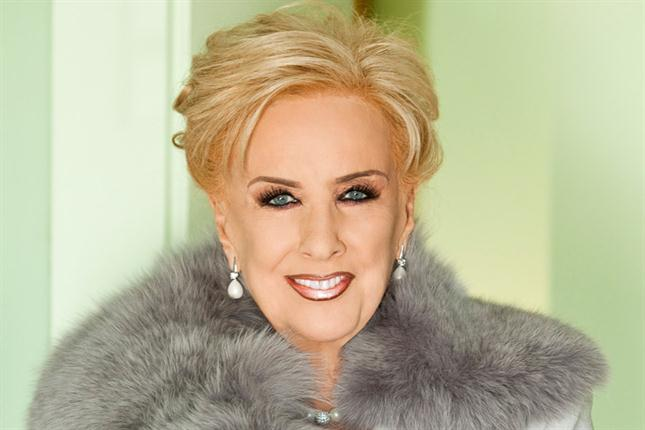
\includegraphics[scale=0.5]{imagenes/mirtha.jpg}
\end{center}
\end{figure}

\setlength{\multicolsep}{0pt}

\subsection{Problema a resolver}

El problema a resolver consiste en salvar a un científico en una ciudad infestada de zombies. Para hacerlo, debemos recorrer la ciudad con una cantidad de soldados iniciales y llegar a un bunker militar. Estos soldados pelean con los zombies que hay en cada calle y mueren según la cantidad de zombies que haya (si hay mas zombies, mueren tantos soldados como el excedente entre la cantidad de zombies y soldados). Queremos que la cantidad de soldados que llegan al bunker sea la máxima posible.

La ciudad en cuestión consiste en calles horizontales y verticales. Cada calle tiene una cantidad variable de zombies.

\medskip
Tenemos los siguientes parámetros de entrada:
\begin{multicols}{2}
	\begin{itemize}[noitemsep,nolistsep]
      \item $n$ = calles horizontales
      \item $m$ = calles verticales
      \item $s$ = soldados iniciales
      \item $pi$ = esquina inicial fila
      \item $pj$ = esquina inicial columna
  	\end{itemize}
\columnbreak
	\begin{itemize}[noitemsep,nolistsep]
      \item $bi$ = esquina bunker fila
      \item $bj$ = esquina bunker columna
      \item $M$ = matriz que le asigna una cantidad $z$ de zombies a cada calle
  	\end{itemize}
\end{multicols}
\medskip

Donde $M$ es una matriz de la pinta:
\begin{itemize}[]
    \item $M$ =
      $
      \begin{pmatrix}
      \begin{matrix} ch_{1,1} & ... & ch_{1,m-1} \end{matrix}\\
      \begin{matrix} cv_{1,1} & & cv_{1,2} & & ... & & cv_{1,m} \end{matrix}\\
      \begin{matrix} ... \end{matrix}\\
      \begin{matrix} cv_{n-1,1} & cv_{n-1,2} & ... & cv_{n-1,m} \end{matrix}\\
      \begin{matrix} ch_{n,1} & ... & ch_{n,m-1} \end{matrix}\\
      \end{pmatrix}
      $
\end{itemize}

Con:
\begin{itemize}[]
  \item $ch_{i,j}$ = \#$\lbrace$ zombies en la calle horizontal i,j $\rbrace$ = \#$\lbrace$ zombies entre las esquinas $v_{i,j}$ y $v_{i,j+1}$ $\rbrace$
  \item $cv_{i,j}$ = \#$\lbrace$ zombies en la calle vertical i,j $\rbrace$ = \#$\lbrace$ zombies entre las esquinas $v_{i,j}$ y $v_{i+1,j}$ $\rbrace$
\end{itemize}

Se atraviesa una calle sin bajas si la cantidad de soldados ($s$) es mayor o igual a $z$. Cuando $z$ es mayor, los soldados sobrevivientes depende del calculo $z$ - $s$. Si esa operación arroja un número mayor o igual a $s$, no hay sobrevivientes, lo que quiere decir que ese camino es inviable.

Por otro lado, queremos resolver este problema de forma que el algoritmo tenga una complejidad de $\mathcal{O}(s*n*m)$. Esto quiere decir que no podemos considerar todos los caminos del punto inicial al bunker. Si ese fuera el caso, la complejidad seria mucho mayor (ver seccion Complejidad). Por eso, es importante considerar la cantidad de soldados al buscar el mejor camino.

\subsection{Resolución planteada}

\subsubsection{Idea y representacion de datos}

Dado que el problema consiste en encontrar un camino entre las esquinas de un mapa con forma de grilla y un costo/zombies en cada calle, parece natural representar el mapa de la ciudad con un grafo.

A su vez, el grafo lo vamos a representar como una matriz de vertices. Cada vertice $v_{i,j}$ corresponde a la esquina del mapa (i,j). Estos tienen la siguiente estructura:

\medskip
\begin{itemize}[noitemsep,nolistsep]
  \item sol_max = maxima cantidad actual de soldados que pueden llegar vivos al vertice
  \item left = costo de ir al vertice de la izquierda, si esto no es posible, un valor que represente a infinito
  \item right = costo de ir al vertice de la derecha, si esto no es posible, un valor que represente a infinito
  \item up = costo de ir al vertice de arriba, si esto no es posible, un valor que represente a infinito
  \item down = costo de ir al vertice de abajo, si esto no es posible, un valor que represente a infinito
  \item pred = vertice desde el cual llegue la ultima vez que actualice sol_max
\end{itemize}
\medskip

Es importante aclarar que como la ciudad es una grilla, cada esquina puede tener a lo sumo cuatro esquinas adyacentes. Entonces me basta guardarme en cada nodo el costo de ir hacia cada una de ellas para no perder ningun arista del grafo representado. A su vez, esto me va a facilitar mucho la manera en la que recorro el grafo, porque toda la informacion que voy a necesitar esta en un mismo lugar.

\medskip

Por ejemplo, sean:

\medskip
\begin{multicols}{3}
  \begin{itemize}[]
      \item $n$ = 3
      \item $m$ = 3
      \item $s$ = 6
    \end{itemize}
\columnbreak
  \begin{itemize}[]
      \item $pi$ = 1
      \item $pj$ = 1
      \item $bi$ = 3
      \item $bj$ = 2
    \end{itemize}
\columnbreak
  \begin{itemize}[]
      \item $M$ =
        $
        \begin{pmatrix}
        \begin{matrix} 1 & 2 \end{matrix}\\
        \begin{matrix}3 & 1 & 2 \end{matrix}\\
        \begin{matrix} 1 & 2 \end{matrix}\\
        \begin{matrix}4 & 1 & 2 \end{matrix}\\
        \begin{matrix} 1 & 2 \end{matrix}\\
        \end{pmatrix}
        $
    \end{itemize}
\end{multicols}
\medskip

Lo comprenderiamos como:

\medskip

% Grafo --------------------------

\begin{centering}

\newarray\data
\readarray{data}{%
1 & 2 &%
3 & 1 & 2 &%
1 & 2 &%
4 & 1 & 2 &%
1 & 2 &%
}%

\grafoCiudad{3}{3}{\data}{1}{1}{3}{2}

\end{centering}

% Grafo --------------------------

\medskip

Donde $BNK$ es la posición del bunker y $ACT$ es la posicion actual, que al principio es donde sale el cientifico con los soldados.

\medskip

Dada toda esta estructura, el algoritmo procede de la forma siguiente: 
Primero, rellena la matriz de vertices con los parametros de entrada. Luego, empezamos a analizar los nodos desde el punto inicial y, mientras el punto analizado $p$ no sea el bunker, calculamos con que cantidad de soldados podemos arribar a los vértices adyacentes (la cuenta correspondiente fue explicada en la seccion previa). \textbf{Solo si} esa cantidad es superior a la maxima cantidad con la que arribamos previamente (dato que contiene el nodo), actualizamos la información del vértice adyacente con la nueva cantidad máxima de soldados, el vértice desde donde se arribo con esa cantidad y pasamos a analizar de forma recursiva el vértice adyacente. Una vez terminado esto analizamos, si es necesario, los demas vecinos de $p$ tambien de forma recursiva. De esta forma recorremos los nodos mediante Backtracking, pero facilitado por el hecho de que solo visitamos los nodos cuando se puede llegar a estos con mas soldados que antes. Por eso, la cantidad de veces que se visita cada nodo esta acotada por la cantidad de soldados iniciales (esto lo vemos bien en la seccion de Complejidad).

\medskip

Por ejemplo, dados los parametros de entrada:

\medskip
\begin{multicols}{3}
  \begin{itemize}[]
      \item $n$ = 3
      \item $m$ = 2
      \item $s$ = 3
    \end{itemize}
\columnbreak
  \begin{itemize}[]
      \item $pi$ = 1
      \item $pj$ = 1
      \item $bi$ = 1
      \item $bj$ = 2
    \end{itemize}
\columnbreak
  \begin{itemize}[]
      \item $M$ =
        $
        \begin{pmatrix}
        \begin{matrix} 5 \end{matrix}\\
        \begin{matrix} 1 & 1 \end{matrix}\\
        \begin{matrix} 4 \end{matrix}\\
        \begin{matrix} 1 & 4 \end{matrix}\\
        \begin{matrix} 1 \end{matrix}\\
        \end{pmatrix}
        $
    \end{itemize}
\end{multicols}
\medskip

Sea $v_{i,j}$ = tupla(int sol_max, tupla(int a, int b) pred) la tupla que usamos para ver el estado de cada nodo en las distintas iteraciones del algoritmo.
Si usamos flechas punteadas para representar desde cual esquina llegue a analizar la actual, el algoritmo procederia asi:

\medskip

% Ejemplo --------------------------

\newarray\data
\readarray{data}{%
5 &%
1 & 1 &%
4 &%
1 & 4 &%
1 &%
}%

\begin{multicols}{2}
\columnbreak
  \grafoCiudad{3}{2}{\data}{1}{1}{1}{2}
\columnbreak
  \begin{itemize}[noitemsep]
      \item[]
      \item $v_{1,1}$ = (3, ($\infty$, $\infty$))
      \item $v_{1,2}$ = (0, ($\infty$, $\infty$))
      \item $v_{2,1}$ = (0, ($\infty$, $\infty$))
      \item $v_{2,2}$ = (0, ($\infty$, $\infty$))
      \item $v_{3,1}$ = (0, ($\infty$, $\infty$))
      \item $v_{3,2}$ = (0, ($\infty$, $\infty$))
    \end{itemize}
\end{multicols}

Aca vemos que desde el nodo $v_{1,1}$ se puede llegar a $v_{1,2}$ y $v_{2,1}$ con mas soldados que antes. El algoritmo entonces hace una llamada recursiva a $v_{1,2}$ con la nueva cantidad de soldados y el nuevo predecesor. Despues de resolver aquel subproblema, se fija si todavia se puede llegar a $v_{2,1}$ con mas soldados que todo lo previamente calculado. El proximo grafico parte de la llamada recursiva a $v_{1,2}$.

\begin{multicols}{2}
\columnbreak
  \grafoCiudadPlus{3}{2}{\data}{1}{2}{1}{2}{
    \draw[-latex,bend right,dash pattern=on3pt off2pt]  (v11) edge (v12);
  }
\columnbreak
  \begin{itemize}[noitemsep]
      \item[]
      \item $v_{1,1}$ = (3, ($\infty$, $\infty$))
      \item $v_{1,2}$ = (1, (1,1))
      \item $v_{2,1}$ = (0, ($\infty$, $\infty$))
      \item $v_{2,2}$ = (0, ($\infty$, $\infty$))
      \item $v_{3,1}$ = (0, ($\infty$, $\infty$))
      \item $v_{3,2}$ = (0, ($\infty$, $\infty$))
    \end{itemize}
\end{multicols}

Se podria llegar con mas soldados a $v_{2,2}$, pero como $v_{1,2}$ es el bunker, dejamos de buscar (ver observacion mas abajo).
Entonces hacemos backtrack a $v_{1,1}$, desde ahi podemos llegar con mas soldados a $v_{2,1}$, asi que procedemos a ese nodo:

\begin{multicols}{2}
\columnbreak
  \grafoCiudadPlus{3}{2}{\data}{2}{1}{1}{2}{
    \draw[-latex,bend right,dash pattern=on3pt off2pt]  (v11) edge (v21);
  }
\columnbreak
  \begin{itemize}[noitemsep]
      \item[]
      \item $v_{1,1}$ = (3, ($\infty$, $\infty$))
      \item $v_{1,2}$ = (1, (1,1))
      \item $v_{2,1}$ = (3, (1,1))
      \item $v_{2,2}$ = (0, ($\infty$, $\infty$))
      \item $v_{3,1}$ = (0, ($\infty$, $\infty$))
      \item $v_{3,2}$ = (0, ($\infty$, $\infty$))
    \end{itemize}
\end{multicols}

Vemos que se puede llegar a $v_{2,2}$ con mas soldados que antes.

\begin{multicols}{2}
\columnbreak
  \grafoCiudadPlus{3}{2}{\data}{2}{2}{1}{2}{
    \draw[-latex,bend right,dash pattern=on3pt off2pt]  (v21) edge (v22);
  }
\columnbreak
  \begin{itemize}[noitemsep]
      \item[]
      \item $v_{1,1}$ = (3, ($\infty$, $\infty$))
      \item $v_{1,2}$ = (1, (1,1))
      \item $v_{2,1}$ = (3, (1,1))
      \item $v_{2,2}$ = (2, (2,1))
      \item $v_{3,1}$ = (0, ($\infty$, $\infty$))
      \item $v_{3,2}$ = (0, ($\infty$, $\infty$))
    \end{itemize}
\end{multicols}

Ahora desde $v_{2,2}$ vamos a proceder a $v_{1,2}$, pero solo porque llegamos con mas soldados que antes. Cuando llegamos al nodo, actualizamos los soldados maximos y el predecesor:

\begin{multicols}{2}
\columnbreak
  \grafoCiudadPlus{3}{2}{\data}{1}{2}{1}{2}{
    \draw[-latex,bend right,dash pattern=on3pt off2pt]  (v22) edge (v12);
  }
\columnbreak
  \begin{itemize}[noitemsep]
      \item[]
      \item $v_{1,1}$ = (3, ($\infty$, $\infty$))
      \item $v_{1,2}$ = (2, (2,2))
      \item $v_{2,1}$ = (3, (1,1))
      \item $v_{2,2}$ = (2, (2,1))
      \item $v_{3,1}$ = (0, ($\infty$, $\infty$))
      \item $v_{3,2}$ = (0, ($\infty$, $\infty$))
    \end{itemize}
\end{multicols}

Despues, hacemos backtrack como antes y desde $v_{2,1}$ vamos a $v_{3,1}$ con mas soldados que antes:

\begin{multicols}{2}
\columnbreak
  \grafoCiudadPlus{3}{2}{\data}{3}{1}{1}{2}{
    \draw[-latex,bend left,dash pattern=on3pt off2pt]  (v21) edge (v31);
  }
\columnbreak
  \begin{itemize}[noitemsep]
      \item[]
      \item $v_{1,1}$ = (3, ($\infty$, $\infty$))
      \item $v_{1,2}$ = (2, (2,2))
      \item $v_{2,1}$ = (3, (1,1))
      \item $v_{2,2}$ = (2, (2,1))
      \item $v_{3,1}$ = (3, (2,1))
      \item $v_{3,2}$ = (0, ($\infty$, $\infty$))
    \end{itemize}
\end{multicols}

Luego procedemos al nodo/esquina $v_{3,2}$:


\begin{multicols}{2}
\columnbreak
  \grafoCiudadPlus{3}{2}{\data}{3}{2}{1}{2}{
    \draw[-latex,bend left,dash pattern=on3pt off2pt]  (v31) edge (v32);
  }
\columnbreak
  \begin{itemize}[noitemsep]
      \item[]
      \item $v_{1,1}$ = (3, ($\infty$, $\infty$))
      \item $v_{1,2}$ = (2, (2,2))
      \item $v_{2,1}$ = (3, (1,1))
      \item $v_{2,2}$ = (2, (2,1))
      \item $v_{3,1}$ = (3, (2,1))
      \item $v_{3,2}$ = (2, (3,1))
    \end{itemize}
\end{multicols}

Ahora desde $v_{3,2}$ no vamos a proceder a $v_{2,2}$ ni ningun otro nodo porque llegariamos con menor o igual cantidad de soldados, esta es la \textbf{clave} para entender la complejidad.
Finalmente, como el nodo $v_{3,2}$ no puede llegar a otro nodo con mas soldados que antes, hacemos backtrack. Como en el backtrack vemos que no podemos llegar a ningun otro nodo con mas soldados que el estado actual, termina la parte principal del algoritmo (solo faltaria reconstruir el camino).

% Ejemplo --------------------------

\medskip

$Observacion$: una vez que llego al bunker, dejo de considerar caminos, es decir, no voy a tratar de llegar a ninguna otra esquina desde el bunker. Esto no nos trae ningun problema porque no existe un camino desde el punto de partida hacia el bunker que pase dos veces por el bunker y sea mejor al sub-camino desde el punto de partida hasta la primera vez que pase por el bunker.

\medskip

De esta forma, reconstruir el camino es facil, dado que tenemos los datos del predecesor de cada nodo y sabemos donde esta el bunker y la posicion inicial (son parametros). Todo lo que habria que hacer es ir recorriendo desde el bunker mediante el predecesor y asi hasta el vertice inicial, agregando los vertices a una pila (asi quedan ordenados del primero al ultimo). Este es el camino que se forma en el ejemplo anterior:

\medskip

\begin{multicols}{2}
\columnbreak
  \grafoCiudadPlus{3}{2}{\data}{1}{1}{1}{2}{
    \node[fill=black!30!green, text=white, align=center, scale=1.5] (v11) at (0, 0) {$v_{11}$};
    \node[fill=black!30!green, text=white, align=center, scale=1.5] (v12) at (2, 0) {$v_{12}$};
    \node[fill=black!30!green, text=white, align=center, scale=1.5] (v21) at (0, -2) {$v_{22}$};
    \node[fill=black!30!green, text=white, align=center, scale=1.5] (v22) at (2, -2) {$v_{22}$};
    \draw[-latex,bend right]  (v11) edge (v21);
    \draw[-latex,bend right]  (v21) edge (v22);
    \draw[-latex,bend right]  (v22) edge (v12);
  }
\columnbreak
  \begin{itemize}[noitemsep]
      \item[]
      \item $v_{1,1}$ = (3, ($\infty$, $\infty$)) = BNK.pred.pred.pred
      \item $v_{1,2}$ = (2, (2,2)) = BNK
      \item $v_{2,1}$ = (3, (1,1)) = BNK.pred.pred
      \item $v_{2,2}$ = (2, (2,1)) = BNK.pred
      \item $v_{3,1}$ = (3, (2,1))
      \item $v_{3,2}$ = (2, (3,1))
    \end{itemize}
\end{multicols}

\medskip

$Observacion$: si no se puede construir un camino, el bunker va a tener como maxima cantidad de soldados 0 y como predecesor ($\infty$, $\infty$). Por eso detectar este caso es simple y no nos produce ningun problema.

\medskip

Como vemos, estamos abarcando de esta manera todos los vértices a los que es posible llegar con los soldados que disponemos en cada caso hasta el bunker. Como vamos a ver en la seccion de Complejidad, visitar los vecinos de un nodo solo cuando se pueda llegar con mas soldados que antes, nos lleva a analizar cada vértice a lo sumo $s$ veces.

\pagebreak

\subsubsection{Pseudocodigo}

\begin{codesnippet}
Sea Esquina una tupla(sol_max:int, left:int, right:int,
        up:int, down:int, predecesor:(int, int))
  con left,...,down la cantidad de zombies entre la esquina y su vecina
  con sol_max la maxima cantidad de zombies actual que pueden llegar a la esquina
  con predecesor la esquina desde donde llegue la ultima vez que actualice sol_max
Sea Mapa un vector(vector(Esquina))
Sea n = calles horizontales
Sea m = calles verticales
Sea s = soldados iniciales
Sea pi = esquina inicial fila
Sea pj = esquina inicial columna
Sea bi = esquina bunker fila
Sea bj = esquina bunker columna
Sea M = matriz que le asigna una cantidad $z$ de zombies a cada calle

Parsear Entrada(n, m, s, pi, pj, bi, bj, M):
  Creamos un mapa llamado map de tamano n*m que es una matriz de vertices

  Inicializamos los vertices de map con los valores de los zombis de cada calle,
  segun corresponda en los campos left, right, up y down,
  sol_max en 0 y predecesor en (INFINITO, INFINITO).
  En caso de no existir un camino a la left, ponemos INFINITO,
  lo mismo para el resto de las posiciones.

  En el campo sol_max de map[pi][pj], ponemos s.

  Luego llamamos la función auxiliar Resolver, con los parámetros mapa,
  posición inicial, posición bunker y, como posicion actual, la inicial.

  Reconstruimos el camino hacia el bunker (si es que existe), es decir, vamos
  desde el bunker recorriendo las esquinas mediante el campo predecesor hasta
  llegar a la posicion inicial y agregando las esquinas a una pila. Finalmente,
  mostramos la solución recorriendo los valores de la pila.

Resolver(map, pi, pj, bi, bj, actuali, actualj):
  Si el vertice <actuali, actualj> es igual a <bi, bj> (el actual es el bunker)
    hago un return
  En caso contrario
    Para cada vecino vcn de map[actuali][actualj] con
        costo (left..down) segun corresponda
    Si puedo ir desde el nodo actual hasta vcn (el costo no es infinito)
    Calculo la cantidad de soldados que llegarian vivos hasta esa esquina
      comparando map[actuali][actualj].sol_max con los zombies en la calle respectiva
      si hay mas soldados o igual cantidad, no muere ninguno
      si hay mas zombies, mueren tantos soldados como el excedente
          entre los zombies y los soldados
    Si ademas puedo llegar hasta vcn con mas soldados que todo lo previamente calculado
      actualizo el campo sol_max de vcn con los sobrevivientes
      actualizo el campo predecesor con la posicion actual
      hago una llamada recursiva a Resolver(map, pi, pj, bi, bj, vcn.fila, vcn.columna)

\end{codesnippet}

\pagebreak

\subsection{Complejidad propuesta}

Dados los parámetros de entrada:

\medskip

\begin{centering}
\begin{multicols}{2}
  \begin{itemize}[noitemsep,nolistsep]
      \item $n$ = calles horizontales
      \item $m$ = calles verticales
      \item $s$ = soldados iniciales
      \item $pi$ = esquina inicial fila
      \item $pj$ = esquina inicial columna
      \item $bi$ = esquina bunker fila
      \item $bj$ = esquina bunker columna
    \end{itemize}
\columnbreak
  \begin{itemize}[noitemsep,nolistsep]
      \item[] Y la matriz de zombies
      \item[]
      \item $M$ =
        $
        \begin{pmatrix}
        \begin{matrix} ch_{1,1} & ... & ch_{1,m-1} \end{matrix}\\
        \begin{matrix} cv_{1,1} & & cv_{1,2} & & ... & & cv_{1,m} \end{matrix}\\
        \begin{matrix} ... \end{matrix}\\
        \begin{matrix} cv_{n-1,1} & cv_{n-1,2} & ... & cv_{n-1,m} \end{matrix}\\
        \begin{matrix} ch_{n,1} & ... & ch_{n,m-1} \end{matrix}\\
        \end{pmatrix}
        $
  \end{itemize}
\end{multicols}
\end{centering}

\medskip

Construimos una matriz de vertices de la forma:

\medskip

\begin{centering}

\readarray{data}{%
$ch_{1,1}$ & & $ch_{1,m-1}$&%
$cv_{1,1}$ & $cv_{1,2}$ & $cv_{1,m-1}$ & $cv_{1,m}$&%
$ch_{2,1}$& &$ch_{2,m-1}$&%
 & & & &%
$ch_{n-1,1}$& &$ch_{n-1,m-1}$&%
$cv_{n-1,1}$ & $cv_{n-1,2}$ & $cv_{n-1,m-1}$ & $cv_{n-1,m}$&%
$ch_{n,1}$ & & $ch_{n,m-1}$&%
}%

\grafoCiudadPlusVacia{4}{4}{\data}{
  % Aristas faltantes
  \path (v41) edge node[below,draw=none,font=\footnotesize] { \data(22) } (v42);
  \path (v42) edge node[below,draw=none,font=\footnotesize] { \data(23) } (v43);
  \path (v43) edge node[below,draw=none,font=\footnotesize] { \data(24) } (v44);
  % Aristas punteados
  \draw[-latex,white,dash pattern=on2pt off2pt, line width=1pt] (v12) edge (v13);
  \draw[-latex,white,dash pattern=on2pt off2pt, line width=1pt] (v22) edge (v23);
  \draw[-latex,white,dash pattern=on2pt off2pt, line width=1pt] (v32) edge (v33);
  \draw[-latex,white,dash pattern=on2pt off2pt, line width=1pt] (v42) edge (v43);
  \draw[-latex,white,dash pattern=on2pt off2pt, line width=1pt] (v21) edge (v31);
  \draw[-latex,white,dash pattern=on2pt off2pt, line width=1pt] (v22) edge (v32);
  \draw[-latex,white,dash pattern=on2pt off2pt, line width=1pt] (v23) edge (v33);
  \draw[-latex,white,dash pattern=on2pt off2pt, line width=1pt] (v24) edge (v34);
  % Nodos Agregados
  \node[fill=white,inner sep=0pt, scale=0.8, minimum size=1.2cm] (v13) at (4, 0) {$v_{1,m-1}$};
  \node[fill=white,inner sep=0pt, scale=0.8, minimum size=1.2cm] (v14) at (6, 0) {$v_{1,m}$};
  \node[fill=white,inner sep=0pt, scale=0.8, minimum size=1.2cm] (v23) at (4, -2) {$v_{2,m-1}$};
  \node[fill=white,inner sep=0pt, scale=0.8, minimum size=1.2cm] (v24) at (6, -2) {$v_{2,m}$};
  \node[fill=white,inner sep=0pt, scale=0.8, minimum size=1.2cm] (v31) at (0, -4) {$v_{n-1,1}$};
  \node[fill=white,inner sep=0pt, scale=0.8, minimum size=1.2cm] (v32) at (2, -4) {$v_{n-1,2}$};
  \node[fill=white,inner sep=0pt, scale=0.7, minimum size=1.2cm] (v33) at (4, -4) {$v_{n-1,m-1}$};
  \node[fill=white,inner sep=0pt, scale=0.8, minimum size=1.2cm] (v34) at (6, -4) {$v_{n-1,m}$};
  \node[fill=white,inner sep=0pt, scale=0.8, minimum size=1.2cm] (v41) at (0, -6) {$v_{n,1}$};
  \node[fill=white,inner sep=0pt, scale=0.8, minimum size=1.2cm] (v42) at (2, -6) {$v_{n,2}$};
  \node[fill=white,inner sep=0pt, scale=0.8, minimum size=1.2cm] (v43) at (4, -6) {$v_{n,m-1}$};
  \node[fill=white,inner sep=0pt, scale=0.8, minimum size=1.2cm] (v44) at (6, -6) {$v_{n,m}$};
}

\end{centering}

\medskip

Como vemos, si en total hay $n$ calles horizontales y $m$ verticales, el total de nodos seria $n*m$. Si representara el grafo como una matriz de adyacencia, solo el costo de cargarla tendria una complejidad mayor a $\mathcal{O}(n*m)$. En cambio, con la forma elegida, solo hay que guardar una cantidad constante de informacion en cada uno de los $n*m$ nodos del grafo.

No podemos considerar todos los caminos del punto inicial al bunker. Si ese fuera el caso, la complejidad seria mucho mayor, ya que la complejidad mencionada recorre cada esquina de la ciudad a lo sumo $s$ veces. Considerando todos los posibles caminos la complejidad seria independiente de $s$, pero la cantidad de veces que analizamos cada una de las $n*m$ esquinas no seria constante. Por ejemplo, si representaramos las $n*m$ esquinas como vertices y las calles como aristas de un grafo y usamos alguna variacion de un algoritmo para hallar caminos minimos como el de Dijkstra, entonces la complejidad quedaria $\mathcal{O}(n^2*m^2)$. Aun optimizandolo con una cola de prioridad la complejidad seguiria siendo $\omega(n*m)$.

Como explicamos anteriormente el algoritmo empieza a analizar los nodos desde el punto inicial y, mientras el punto analizado $p$ no sea el bunker, calcula con que cantidad de soldados podemos arribar a los vértices adyacentes. La forma en que recorre los nodos es parecida a Backtracking, prioriza la profundidad del camino, pero dada una esquina, solo hace una llamada recursiva a un nodo vecino cuando podemos llegar a el con mas soldados que todos los caminos antes calculados.
Lo importante de este procedimiento es el hecho de que cada uno de los $n*m$ nodos es analizado cuando se puede llegar al nodo con una cantidad de soldados mayor a la previamente calculada. Es decir, si yo llegue a un nodo con $k$ soldados, ese nodo no se volvera a analizar con una cantidad de soldados menor o igual a $k$. Entonces, como uno empieza el algoritmo con $s$ soldados y la cantidad de soldados no puede aumentar (solo disminuir o quedar fija), a lo sumo se visita cada nodo con 1, 2, ... , $s$ soldados en ese orden. Entonces, a diferencia de un Backtracking normal, cada nodo puede ser visitado a lo sumo $s$ veces.

Aparte de lo ya mencionado, el algoritmo tambien tiene que reconstruir el camino de la posicion inicial al bunker (si es que existe) e imprimirlo. De todas maneras, esto se resuelve facilmente recorriendo las esquinas desde el bunker hasta el punto inicial con el campo de predecesor que cada una contiene. Mientras visitamos los vertices, los vamos guardando en una pila (pues los queremos imprimir en el orden inverso) y luego los imprimimos. Como a lo sumo pasamos una vez por cada uno de los vertices y hay $n*m$ de ellos, este paso tiene complejidad $\mathcal{O}(n*m)$.

Por lo tanto, vimos que el grafo en cuestion tiene $n*m$ nodos y cargarlo tanto como imprimirlo al final cuesta $\mathcal{O}(n*m)$. Ademas, como cada nodo tiene a lo sumo cuatro vecinos y por cada uno de ellos el algoritmo solo hace comparaciones para saber si hay que analizarlo, podemos decir que se realiza trabajo constante (ademas de las llamadas recursivas) en cada paso de la recursion. Entonces dado que el algoritmo pasa por cada nodo a lo sumo $s$ veces, son $n*m$ nodos y realiza trabajo constante en cada uno, concluimos que la complejidad del algoritmo es $\mathcal{O}(s*n*m)$.

\newpage
\subsection{Implementación en C++}
\lstinputlisting[language=C++, breaklines]{codigo/ej2.cpp}

\newpage
\subsection{Experimentación computacional}

%Esto sirve para arreglar la posicion de los labels en los graficos
\pgfplotsset{compat=1.5}

Consideraciones:
\begin{itemize}
  \item Todos los experimentos fueron hechos bajo las mismas condiciones (computadora, procesos abiertos, alimentacion, etc..)
  \item Para cada medicion exactamente igual se tomaron 20 pruebas, los valores que aparecen en los graficos son los del promedio entre las diferentes corridas.
  \item Se midieron los tiempos con la biblioteca chrono y estos fueron convertidos a nanosegundos.
  \item Los valores aleatorios que fuimos tomando en algunos de los experimentos fueron tomados con una distribucion uniforme para el rango requerido.
  \item Tomamos entre 100 y 200 valores de entrada diferente en cada experimento. Por ejemplo, si el tamano de entrada va de 1 a 5000, mediriamos los valores con tamano de entrada 1, 50, 100, 150, ..., 5000. Esto sirve para no sobrepopular los graficos.
  \item Salvo indicado lo contrario, la posicion inicial del cientifico y la posicion del bunker van a ser aleatorias (si bien en un rango valido).
  \item Vamos a querer medir la rapidez del algoritmo segun los parametros:
    \begin{itemize}
      \item $n$ = calles horizontales
      \item $m$ = calles verticales
      \item $s$ = soldados iniciales
      \item y la cantidad de zombies en cada esquina
    \end{itemize}
  \item Vamos a querer mostrar que el algoritmo funciona como explicamos y que el trabajo que realiza se condice con nuestra cota analizada en la seccion de Complejidad. Nuestra cota fue $\mathcal{O}(s*n*m)$.
\end{itemize}

\subsubsection{Experimentación con instancias aleatorias}

En esta seccion, realizamos una serie de experimentos donde la cantidad de zombies en cada calle es aleatoria. Para probar la eficiencia del algoritmo vamos fijando algunos parametros de entrada y variando los otros. Si bien la cantidad de zombies va a ser aleatoria, su rango de valores posibles va a estar entre 0 y $2*s$ (dos veces la cantidad de soldados iniciales). Esto es importante y necesario pues si no lo hicieramos asi, los soldados serian destruidos por los zombies muy rapidamente, ya que habria una cantidad de zombies enorme en cada calle en comparacion a los soldados.

\paragraph{Experimento 1}

Para el primer experimento, vamos a variar los parametros de entrada $s$, $n$ y $m$ uniformemente. Es decir, el tamano de entrada es una variable $L$ donde $s=n=m=L$ que se va incrementando. Los valores de $L$ van a variar entre 1 y 200. Vamos a querer ver que nuestra cota de complejidad es $\mathcal{O}(L^3)=\mathcal{O}(L*L*L)=\mathcal{O}(s*n*m)$. Veamos los resultados:

%Grafico
\graficarDatos
{s, n, m variables}
{$L$}{Tiempo de ejecucion (nanosegundos)}
{s*n*m}{tiempo}
{datos/ej2-04.dat}

El grafico tiene cierta pendiente que es claramente no lineal. Queremos ver que es una pendiente como la de una funcion $f(L)=L^3$.Si dividimos los tiempos por $L$, tenemos el siguiente grafico:

%Grafico
\graficarDatos
{s, n, m variables, divido los tiempos originales por $L$}
{$L$}{Tiempo de ejecucion (nanosegundos) / $L$}
{s*n*m}{tiempo}
{datos/ej2-042.dat}

Dividiendo por segunda vez los tiempos por $L$ nos queda:

%Grafico
\graficarDatos
{s, n, m variables, divido los tiempos originales por $L^2$}
{$L$}{Tiempo de ejecucion (nanosegundos) / $L^2$}
{s*n*m}{tiempo}
{datos/ej2-043.dat}

Esto ultimo parece ser lineal, lo que seria un indicio que estabamos en lo correcto y la complejidad del algoritmo sigue la curva de una funcion tal como $f(L)=L^3$. Veamos el grafico que queda si dividimos los tiempos por $L$ una vez mas:

%Grafico
\graficarDatosPlus
{s, n, m variables, divido los tiempos originales por $L^3$}
{$L$}{Tiempo de ejecucion (nanosegundos) / $L^3$}
{s*n*m}{tiempo}
{datos/ej2-044.dat}
{restrict y to domain = 0:100}

La pendiente tiende a una constante por arriba del 0. Esto quiere decir que estabamos en lo correcto, ya que la funcion sigue una curva al estilo cubico. Entonces se condice con nuestra cota de complejidad $\mathcal{O}(s*n*m)$, pues fijamos $s=n=m=L$ y nos quedo un grafico que sigue la curva de una funcion polinomial de grado 3.

\paragraph{Experimento 2}

Para este experimento, fijamos los valores de $n$ y $m$ en 20 mientras variamos los valores de $s$, los resultados fueron:

%Grafico
\graficarDatos
{n=20, m=20, s variable}
{s (cantidad de soldados)}{Tiempo de ejecucion (nanosegundos)}
{s}{tiempo}
{datos/ej2-01.dat}

Esto pareceria ser lineal desde la segunda mitad del dominio, veamos que pasa cuando dividimos los tiempos por el tamano de entrada $s$:

%Grafico
\graficarDatosPlus
{n=20, m=20, s variable, divido los tiempos por s}
{s (cantidad de soldados)}{Tiempo de ejecucion (nanosegundos) / s}
{s}{tiempo}
{datos/ej2-012.dat}
{ymin=75000, ymax=400000}

Parece que la pendiente se vuelve constante y la constante a la que tiende esta por arriba del 0. Esto se condice con nuestra cota de complejidad $\mathcal{O}(s*n*m)$, pues fijamos $n=20, m=20$ y el tiempo varia linealmente con respecto a $s$.

\paragraph{Experimento 3}

En este experimento, fijamos los valores de $m$ en 100 y $s$ en 10000 mientras variamos los valores de $n$, los resultados fueron:

%Grafico
\graficarDatos
{n variable, m=100, s=10000}
{n (cantidad de calles horizontales)}{Tiempo de ejecucion (nanosegundos)}
{n}{tiempo}
{datos/ej2-02.dat}

Tiene una clara pinta de lineal, veamos lo que pasa cuando dividimos los tiempos por el tamano de entrada $n$:

%Grafico
\graficarDatosPlus
{n=100, m variable, s=10000, divido los tiempos por n}
{n (cantidad de calles horizontales)}{Tiempo de ejecucion (nanosegundos) / n}
{n}{tiempo}
{datos/ej2-022.dat}
{ymax=20000, ymin=5000}

Como vemos, la pendiente tiende a una constante por arriba del 0. Esto se condice con nuestra cota de complejidad $\mathcal{O}(s*n*m)$, pues fijamos $m=100, s=10000$ y el tiempo varia linealmente con respecto a $n$.

\paragraph{Experimento 4}

Fijamos los valores de $n$ en 100 y $s$ en 10000 mientras variamos los valores de $m$, los resultados fueron:

%Grafico
\graficarDatos
{n=100, m variable, s=10000}
{m (cantidad de calles verticales)}{Tiempo de ejecucion (nanosegundos)}
{m}{tiempo}
{datos/ej2-03.dat}

Es muy parecido al experimento anterior. La curva parece lineal, veamos lo que pasa cuando dividimos los tiempos por el tamano de entrada $m$:

%Grafico
\graficarDatosPlus
{n=100, m variable, s=10000, divido los tiempos por m}
{m (cantidad de calles verticales)}{Tiempo de ejecucion (nanosegundos) / m}
{m}{tiempo}
{datos/ej2-032.dat}
{ymax=20000, ymin=5000}

Esta pendiente tambien tiende a una constante por arriba del 0. Esto se condice con nuestra cota de complejidad $\mathcal{O}(s*n*m)$, pues fijamos $n=100, s=10000$ y el tiempo varia linealmente con respecto a $m$.

\subsubsection{Experimentación con instancias particulares}

Cuando analizamos instancias particulares, nos va a interesar fijar la cantidad de zombies en cada calle al contrario que las instancias aleatorias. A la vez vamos a ir variando ciertos parametros de entrada. 

\paragraph{Experimento 1: Mejor caso 1}

En este caso vamos a fijar la cantidad de zombies en cada calle a 0. Variamos los parametros de entrada $n$ y $m$ uniformemente y dejamos la cantidad de soldados fija en 1000:

%Grafico
\graficarDatos
{n, m variables}
{n, m (son iguales)}{Tiempo de ejecucion (nanosegundos)}
{e}{tiempo}
{datos/ej2-11.dat}

Dividiendo por $n$ nos queda:

%Grafico
\graficarDatos
{n, m variables}
{n, m (son iguales)}{Tiempo de ejecucion (nanosegundos) / n}
{e}{tiempo}
{datos/ej2-112.dat}

Esto es algo de pinta lineal. Si dividimos por $m$ nos queda:

%Grafico
\graficarDatosPlus
{n, m variables}
{n, m (son iguales)}{Tiempo de ejecucion (nanosegundos) / n}
{e}{tiempo}
{datos/ej2-113.dat}
{restrict y to domain = 0:1000}

Que tiende a una constante por encima de 0. Esto se condice con nuestra cota de complejidad $\mathcal{O}(s*n*m)$, pues fijamos $s$ y el tiempo varia linealmente con respecto a $n*m$.

\paragraph{Experimento 2: Mejor caso 2}

Como antes, la cantidad de zombies en cada calle va a ser 0. Pero a diferencia del caso anterior, fijamos los parametros $n$ y $m$ en 100 y variamos la cantidad de soldados:

%Grafico
\graficarDatosPlus
{n=100, m=100, s variable}
{s}{Tiempo de ejecucion (nanosegundos)}
{s}{tiempo}
{datos/ej2-13.dat}
{ymin=0, ymax=3000000}

Si bien la cantidad de soldados varia en un rango muy grande, el tiempo no varia demasiado. Esto tiene sentido ya que tenemos la misma cantidad de esquinas para llegar pero siempre llegamos una vez sola. Es decir, como la cantidad de zombies en cada calle es 0, solo llego a cada esquina una vez (con la maxima cantidad de soldados posibles). Esto se condice con nuestra explicacion sobre la forma en que funciona el algoritmo.

\paragraph{Experimento 3: Peor caso}

Generar una instancia con uno de los peores casos no es simple. En este caso, vamos a generar un peor caso analizando el codigo del algoritmo. Este hace Backtracking y analiza las posibilidades en el orden: izquierda, derecha, arriba, abajo. Vamos a hacer una instancia donde maximizemos la cantidad de veces que pasamos por cada esquina. Sea $k$ una variable, vamos a configurar $n=2k, m=2k$ e ir variando $s$ entre 1 y $k$. Ademas vamos a tener las siguientes cantidades de zombies:

\newarray\data
\readarray{data}{%
$2k$ & 1 & 1&%
1 & 1 & 1 & 1&%
$2k-1$ & 1 & 1&%
 & & & &%
$2$ & 1 & 1&%
1 & 1 & 1 & 1&%
$1$ & 1 & 1&%
}%

\begin{centering}

\grafoCiudadPlusVacia{4}{4}{\data}{
  % Aristas faltantes
  \path (v41) edge node[below,draw=none,font=\footnotesize] { \data(22) } (v42);
  \path (v42) edge node[below,draw=none,font=\footnotesize] { \data(23) } (v43);
  \path (v43) edge node[below,draw=none,font=\footnotesize] { \data(24) } (v44);
  % Aristas punteados
  \draw[-latex,white,dash pattern=on2pt off2pt, line width=1pt] (v12) edge (v13);
  \draw[-latex,white,dash pattern=on2pt off2pt, line width=1pt] (v22) edge (v23);
  \draw[-latex,white,dash pattern=on2pt off2pt, line width=1pt] (v32) edge (v33);
  \draw[-latex,white,dash pattern=on2pt off2pt, line width=1pt] (v42) edge (v43);
  \draw[-latex,white,dash pattern=on2pt off2pt, line width=1pt] (v21) edge (v31);
  \draw[-latex,white,dash pattern=on2pt off2pt, line width=1pt] (v22) edge (v32);
  \draw[-latex,white,dash pattern=on2pt off2pt, line width=1pt] (v23) edge (v33);
  \draw[-latex,white,dash pattern=on2pt off2pt, line width=1pt] (v24) edge (v34);
  % Nodos Agregados
  \node[fill=white,inner sep=0pt, scale=0.8, minimum size=1.2cm] (v13) at (4, 0) {$v_{1,m-1}$};
  \node[fill=white,inner sep=0pt, scale=0.8, minimum size=1.2cm] (v14) at (6, 0) {$v_{1,m}$};
  \node[fill=white,inner sep=0pt, scale=0.8, minimum size=1.2cm] (v23) at (4, -2) {$v_{2,m-1}$};
  \node[fill=white,inner sep=0pt, scale=0.8, minimum size=1.2cm] (v24) at (6, -2) {$v_{2,m}$};
  \node[fill=white,inner sep=0pt, scale=0.8, minimum size=1.2cm] (v31) at (0, -4) {$v_{n-1,1}$};
  \node[fill=white,inner sep=0pt, scale=0.8, minimum size=1.2cm] (v32) at (2, -4) {$v_{n-1,2}$};
  \node[fill=white,inner sep=0pt, scale=0.7, minimum size=1.2cm] (v33) at (4, -4) {$v_{n-1,m-1}$};
  \node[fill=white,inner sep=0pt, scale=0.8, minimum size=1.2cm] (v34) at (6, -4) {$v_{n-1,m}$};
  \node[fill=white,inner sep=0pt, scale=0.8, minimum size=1.2cm] (v41) at (0, -6) {$v_{n,1}$};
  \node[fill=white,inner sep=0pt, scale=0.8, minimum size=1.2cm] (v42) at (2, -6) {$v_{n,2}$};
  \node[fill=white,inner sep=0pt, scale=0.8, minimum size=1.2cm] (v43) at (4, -6) {$v_{n,m-1}$};
  \node[fill=white,inner sep=0pt, scale=0.8, minimum size=1.2cm] (v44) at (6, -6) {$v_{n,m}$};
}

\end{centering}

Es decir, todas las calles van a tener 1 zombie excepto la primer calle horizontal de cada fila, estas van a tener $2k, 2k-1, 2k-2, ..., 3, 2, 1$ zombies en ese orden.
Ademas, vamos a fijar la posicion inicial del cientifico en (0,0) y la posicion del bunker en la esquina de abajo a la derecha, garantizando que el ejemplo funcione bien.
Como el algoritmo analiza ir hacia los nodos vecinos en el orden: izquierda, derecha, arriba y abajo, va a llenar casi todos los nodos de la matriz con un 1, luego con un 2, despues con un 3 y asi hasta $s$.
Seteando $k=50$, los resultados fueron los siguientes:

%Grafico
\graficarDatos
{k=50, s variable entre 1 y k}
{s}{Tiempo de ejecucion (nanosegundos)}
{s}{tiempo}
{datos/ej2-12.dat}

Como esto tiene pinta de lineal en $s$, dividimos los tiempos por $s$:

%Grafico
\graficarDatosPlus
{k=50, s variable entre 1 y k, dividimos los tiempo por $s$}
{s}{Tiempo de ejecucion (nanosegundos) / s}
{s}{tiempo}
{datos/ej2-122.dat}
{ymin=1000000, ymax=2000000}

Y esto parece tender a una constante por encima de 0. Por lo tanto esto se condice con nuestra cota de complejidad porque aun en uno de los peores casos, el tiempo que tarda el algoritmo varia linealmente con respecto a $s$.

\newpage
\section{Ejercicio 3 - Refinando petróleo}
\begin{figure}[h]
\begin{center}
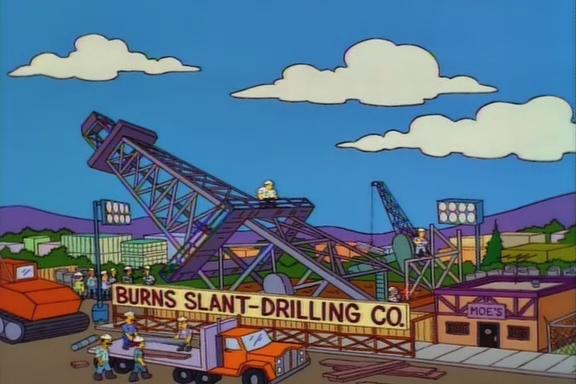
\includegraphics[width=0.6\textwidth] {imagenes/burnsoil.JPG}
\end{center}
\end{figure}

\subsection{Problema a resolver}
El problema a resolver consiste en encontrar un algoritmo que dé un plan de acción para construir una cantidad de refinerías y tuberías entre pozos de petroleo con costo mínimo. Para esto se provee una cantidad de pozos de petroleo, una cantidad de tuberías que se pueden construir entre dos pozos y un costo fijo de poner una refinería en un pozo dado. \\
Se debe encontrar, con el menor costo posible, un plan indicando cuales son las refinerías y tuberías a construir en el que, o bien todas los pozos tengan una refinería, o bien estén conectados a una mediante una o un conjunto de tuberías.

\smallskip
Tenemos los siguientes parámetros de entrada:
	\begin{itemize}[noitemsep,nolistsep]
      \item $n$ = Cantidad de pozos
      \item $m$ = Cantidad de tuberías posibles
      \item $c$ = Costo por refinería
      \item Luego vienen $m$ líneas con tuberías donde $T_{i}$ representa a la tubería en la línea $i$ con $1 \leq i \leq m$ y tiene los siguientes parámetros:
      \begin{itemize}
      \item $o_{i}$ = Tubería de orígen
      \item $d_{i}$ = Tubería de destino
      \item $c_{i}$ = Costo de la tubería
      \end{itemize}
  	\end{itemize}
\smallskip

\subsection{Resolución planteada}
Para resolver este problema, modelaremos la entrada con un grafo, en donde cada pozo es un nodo y cada tubería que podemos construir es una arista con el costo de la construcción de la misma. \\

\begin{itemize}
\item Ejemplo 1:

Sean:
\begin{itemize}
      \item $n$ = 7
      \item $m$ = 6
      \item $c$ = 3
\end{itemize}

Y luego $m$ tuberías:

\begin{table}[H]
\centering
\parbox{0.3\textwidth}{
    \begin{tabular}{ | l | l | l | l |}
    \hline
$T_{i}$ & $o_{i}$ & $d_{i}$ & $c_{i}$ \\ \hline
$T_{1}$ & 1 & 2 & 1 \\ \hline
$T_{2}$ & 3 & 4 & 1 \\ \hline
$T_{3}$ & 2 & 3 & 2 \\ \hline
$T_{4}$ & 1 & 4 & 3 \\ \hline
$T_{5}$ & 5 & 6 & 2 \\ \hline
$T_{6}$ & 2 & 7 & 4 \\ \hline
    \end{tabular}
}
\end{table}

Ésta entrada particular la comprenderíamos con el siguiente grafo:

\tikz[every node/.style={draw,circle}] {
\node (1) at (0, 0)  { 1 };
\node (2) at (2, 0)  { 2 };
\node (3) at (2,-2)  { 3 };
\node (4) at (0,-2)  { 4 };
\node (5) at (4, 0)  { 5 };
\node (6) at (5,-2)  { 6 };
\node (7) at (3,-1)  { 7 };
\draw (1) edge node[above,draw=none] { 1 } (2);
\draw (3) edge node[above,draw=none] { 1 } (4);
\draw (2) edge node[left,draw=none] { 2 } (3);
\draw (1) edge node[left,draw=none] { 3 } (4);
\draw (5) edge node[above,draw=none] { 2 } (6);
\draw (2) edge node[above,draw=none] { 4 } (7);
}

Y una solución válida (no es única) para el siguiente caso se representaría con el siguiente grafo:

\tikz[every node/.style={draw,circle}] {
\node[fill=red!40, text=white] at (3,-1) {7};
\node[fill=red!40, text=white] at (0,0) {1};
\node[fill=red!40, text=white] at (4,0) {5};
\node[fill=blue!40, text=white] at (2,0) {2};
\node[fill=blue!40, text=white] at (2,-2) {3};
\node[fill=blue!40, text=white] at (0,-2) {4};
\node[fill=blue!40, text=white] at (5,-2) {6};
\draw (1) edge[green] node[above,draw=none] { 1 } (2);
\draw (3) edge[green] node[above,draw=none] { 1 } (4);
\draw (2) edge[green] node[left,draw=none] { 2 } (3);
%\draw (1) edge node[left,draw=none] { 3 } (4);
\draw (5) edge[green] node[above,draw=none] { 2 } (6);
%\draw (2) edge node[above,draw=none] { 4 } (7);
}

Donde los nodos rojos representan pozos con refinería, los ejes verdes representan las tuberías que fueron construidas y los nodos azules representan pozos que no tienen una refinería pero están conectadas a una por ejes verdes.
\end{itemize}

Ahora, observemos lo siguiente. Si yo tengo dos pozos unidos por una posible tubería y ésta tiene costo mayor al costo de poner una refinería, entonces esa tubería nunca estará construida en la solución.
Por ejemplo:
\begin{itemize}
\item Ejemplo 2:

Sean:
\begin{itemize}
      \item $n$ = 2
      \item $m$ = 1
      \item $c$ = 3
\end{itemize}

Y luego $m$ tuberías:

\begin{table}[H]
\centering
\parbox{0.3\textwidth}{
    \begin{tabular}{ | l | l | l | l |}
    \hline
$T_{i}$ & $o_{i}$ & $d_{i}$ & $c_{i}$ \\ \hline
$T_{1}$ & 1 & 2 & 5 \\ \hline
    \end{tabular}
}
\end{table}

Esta entrada particular la comprenderíamos con el siguiente grafo:

\tikz[every node/.style={draw,circle}] {
\node (1) at (0, 0)  { 1 };
\node (2) at (2, 0)  { 2 };
\draw (1) edge node[above,draw=none] { 5 } (2);
}

En este caso, construyendo la tubería, el grafo solución sería el siguiente:

\tikz[every node/.style={draw,circle}] {
\node[fill=red!40, text=white] at (0,0) {1};
\node[fill=blue!40, text=white] at (2,0) {2};
\draw (1) edge[green] node[above,draw=none] { 5 } (2);
}

Acá tendríamos un costo total de 8 (una refinería con costo 3 más la tubería con costo 5).

Sin embargo,la solución correcta sería la siguiente:

\tikz[every node/.style={draw,circle}] {
\node[fill=red!40, text=white] at (0,0) {1};
\node[fill=red!40, text=white] at (2,0) {2};
}

Donde el costo total sería 6 (dos refinerías de costo 3)
\end{itemize}



Y esto lo podemos generalizar: \\

\begin{lemma}
        sean dos componentes conexas $C_{1}$ y $C_{2}$ con las tuberías necesarias construidas para garantizar un costo mínimo, y sea $T$ una posible tubería entre un pozo en $C_{1}$ y uno en $C_{2}$. $T$ solo será construída en una solución de costo mínimo si su costo es menor o igual al costo de la refinería.
    \end{lemma}

\begin{proof}
Sea $costo()$ la función que recibe un conjunto de pozos y tuberías construidas y devuelve el costo total de la construcción. \\

Sea $c$ el costo de una refinería.

Una componente conexa que está en una solución válida tiene costo mínimo, por ende, sólo tiene una refinería en ella porque en caso de tener un pozo que este conectado a una refinería por tuberías, y que a su vez tenga una refinería en el pozo, ésta no sería una solución mínima ya que puedo eliminar esa refinería reduciendo el costo total y el pozo seguiría estando conectado con una.

Ahora, sean dos componentes conexas $C_{1}$ y $C_{2}$ con las tuberías necesarias construidas para garantizar un costo mínimo, y sea $T$ una posible tubería entre un pozo en $C_{1}$ y uno en $C_{2}$.

El costo de la tubería $T$ es $costo(T)$.

Mi costo acumulado de $C_{1}$ y $C_{2}$ es $costo(C_{1})$ y $costo(C_{2})$ respectivamente.

Como estamos buscando minimizar el costo, $T$ debe ser construida si se da lo siguiente:

$$costo(C_{1}) + costo(C_{2}) \geq costo(C_{1}) + costo(C_{2}) + costo(T) - c$$

Entonces, despejando, solo debe ser construida si:

$$c \geq costo(T)$$
\end{proof}

Por lo tanto, ya que una tubería con costo mayor al de una refinería nunca va a ser construida, podríamos no agregarla al modelar la entrada en un grafo. En el ejemplo 1, el grafo quedaría de la siguiente manera:

\tikz[every node/.style={draw,circle}] {
\node (1) at (0, 0)  { 1 };
\node (2) at (2, 0)  { 2 };
\node (3) at (2,-2)  { 3 };
\node (4) at (0,-2)  { 4 };
\node (5) at (4, 0)  { 5 };
\node (6) at (5,-2)  { 6 };
\node (7) at (3,-1)  { 7 };
\draw (1) edge node[above,draw=none] { 1 } (2);
\draw (3) edge node[above,draw=none] { 1 } (4);
\draw (2) edge node[left,draw=none] { 2 } (3);
\draw (1) edge node[left,draw=none] { 3 } (4);
\draw (5) edge node[above,draw=none] { 2 } (6);
}

Entonces, de ahora en adelante modelaremos la entrada en un grafo, pero solo añadiremos como aristas las tuberías que tengan costo menor al costo de la refinería. \\

Notemos que podemos dividir nuestro problema en un subproblema por cada componente conexa que tenga nuestra entrada. \\

Necesitamos entonces, encontrar una solución mínima en cada componente conexa. Notemos ahora que si una componente conexa está en el modelo, entonces existe una solución con una sola refinería para toda la componente, ya que se puede llegar de cualquier pozo a cualquier otro mediante tuberías posibles y que todas las tuberías tienen costo menor al costo de una refinería. Notemos también que la solución no tendrá ciclos, ya que de tenerlos, ésta solución no sería mínima porque se podría eliminar una tubería perteneciente al ciclo, reduciendo el costo total de la construcción y aún así se podría llegar de cualquier nodo de la componente a cualquier otro mediante tuberías. \\

Sacando en limpio estos datos, lo que estamos buscando en cada componente es encontrar una solución que recorra todos los nodos de la componente, es decir, que sea conexa, que no tenga ciclos, y que a la vez tenga costo mínimo. Entonces, lo que estamos buscando es encontrar el árbol generador mínimo de cada componente conexa. \\

Ahora, si encuentro un árbol generador mínimo de cada componente conexa del grafo con el que modelamos la entrada, estaría consiguiendo una solución con costo mínimo. Entonces, lo que el problema realmente nos está pidiendo es encontrar un bosque generador mínimo del grafo, ya que debemos minimizar los costos de la construcción de refinerías y tuberías. \\

Para resolver el siguiente problema, usaremos el algoritmo de Kruskal. \\
Dado un grafo, el algoritmo de Kruskal se encarga de encontrar el árbol generador mínimo en el mismo, y en caso de no ser posible porque el grafo tiene más de una componente conexa, el algoritmo encuentra el bosque generador mínimo. \\
\\
El algoritmo de Kruskal, ordena primero las aristas del grafo según su costo en una estructura y luego recorre la misma en orden fijándose por cada arista si los dos nodos pertenecen a la misma componente, si estos no pertenecen a la misma componente, agrega la arista y une las componentes, y si pertenecen a la misma componente desestima esa arista ya que ya están conectadas. \\
\\
De esta forma, al finalizar de recorrer la estructura quedarían tantos árboles como componentes conexas tiene el grafo, como estos árboles tienen costo mínimo, el bosque resultante es el bosque generador mínimo.  \\
\\
En nuestro caso, usaremos como estructura una cola de prioridad que priorice por menor costo. Además, para modelar el grafo correctamente, solo añadiremos a la cola de prioridad las tuberías posibles que tengan costo menor al costo de construir una refinería.


\subsubsection{Pseudocódigo}

Pseudocódigo de la solución

\begin{codesnippet}
//Creamos un entero con el costo de crear una refinería en cada pozo
int costoTotal <- n*m

//Creo una cola de prioridad
ColaPrior tuberías

//Sea t el conjunto con las tuberías que se reciben en el input
//Encolamos en la cola de prioridad las tuberías de t con costo menor a c
Por cada tubería i de las m posibles que se ingresan en t
	Si el costo de la tubería i es menor a c
    	tuberías.encolar(t[i])
    Fin si
Fin por

//Creamos un vector de tuberías donde guardare las tuberías que se construyen
Vector tuberíasConstruidas

//Creamos un conjunto disjunto con los pozos
UnionFind componentes(n)

Mientras tuberías no este vacío
  //Sea top el primer elemento de la colaPrior tuberías
  	top <- tuberías.primero()

    Si el origen de la tuberías top no esta en el mismo conjunto que el destino
      //Unimos los conjuntos a los que pertenecen ambos pozos
        componentes.unir(top.origen,top.destino)

        //Agregamos a top al vector de tuberías construidas
        tuberíasConstruidas.agregarAtras(top)

        //Bajamos el costo total
        costoTotal <- costoTotal - c + top.costo
    Fin si

    //Desencolamos a top de la cola de prioridad
    tuberías.desencolar()
Fin mientras

//Ahora solo resta mostrar la solución
Mostramos costoTotal, la cantidad de conjuntos que tiene componentes y
el tamaño de tuberíasConstruidas

//Mostramos un elemento de cada conjunto de componentes
Por cada conjunto en componentes
	mostrar el primer elemento
Fin por

//Mostramos las tuberías construidas
Por cada tubería i en tuberíasConstruidas
	mostrar tuberíasConstruidas[i]
Fin por
\end{codesnippet}
Pseudocódigo de la estructura UnionFind: \\

\begin{codesnippet}
Vamos a representar cada conjunto como un árbol.
Tengo dos arreglos de tamaño n, uno que representa el id al que pertenece el elemento i,
con i entre 0 y n. Y el otro representa el rank del elemento i.
El id lo que indica es quien es la raíz del árbol al que pertenece el elemento.
A la vez, tengo un entero llamado cantidadDeArboles que tiene tamaño n al inicializar.

//devuelve la raiz del arbol a la que pertenece un elemento
buscar(p)
  raiz = p
  mientras raiz != id[raiz]
  	raiz = id[raiz]
  mientras p != raiz
  	newp = id[p]
  	id[p] = raiz
  	p = newp

  return raiz

//une dos componentes
unir(x, y)
  i = buscar(x)
  j = buscar(y)

  //si son iguales ya estaban en la misma componente
  si i == j return

  //hace que la raiz del menor apunte a la del mayor
  si rank[i] < rank[j]
    id[i] = j
  sino
   id[j] = i
   si rank[i] == rank[j]
    rank[i]++;


  cantidadDeArboles--;


//devuelve true si dos elementos estan en el mismo arbol
conectados(x,y)
   return buscar(x) == buscar(y);


count()
	return cantidadDeArboles;

\end{codesnippet}



\subsection{Complejidad propuesta}

Como se ve en el pseudocódigo, la solución al problema se divide en tres partes, que son guardar los datos de entrada, encontrar la solución y mostrarla. El enunciado nos pide resolver todo en una complejidad estrictamente menor a  $\mathcal{O}(n^{3})$. \\

Al procesar la entrada, se guardan $n$, $m$ y $c$ en $\mathcal{O}(1)$, se crea un UnionFind con n conjuntos en $\mathcal{O}(n)$, y luego se guardan las tuberías posibles con costo menor a $c$ en una cola de prioridad. Las tuberías son a lo sumo $m$ y encolar cada una tiene costo $\mathcal{O}(log(m))$. Por lo tanto, todo el proceso de guardar los datos de entrada tiene complejidad $\mathcal{O}(m*log(m))$, y como $m$ está acotado superiormente por $n^2$, la complejidad sería $\mathcal{O}(n^2*log(n))$. \\

Veamos ahora la complejidad de encontrar la menor solución. Esto se realiza en un ciclo definido por el tamaño de la cola de prioridad, que es a lo sumo $m$. Dentro del ciclo, se guarda el primer elemento de la cola, esto se realiza en $\mathcal{O}(1)$. Luego se revisa si ambas tuberías pertenecen al mismo conjunto del UnionFind, de no ser así, estas se unen. \\

Entonces, por cada tubería, tengo a lo sumo que llamar dos veces a la función buscar y una vez a la función unir del UnionFind. \\

Si la tubería es construida, además de unir en el UnionFind, se debe agregarla al vector que guarda las tuberías construidas, y esto se hace en $\mathcal{O}(1)$. También, se debe bajar el costo total de la construcción que también es $\mathcal{O}(1)$.

Como podemos ver en el pseudocódigo, nuestro UnionFind utiliza las dos heurísticas para UnionFind implementado sobre árboles. Éstas son union by rank y path compression.

La heurística path compression está implementada en la función buscar y lo que hace es que al buscar un elemento, les actualiza no solo a el elemento sino a todos sus padres la raíz a la raíz del árbol. Esto hace que en llamados posteriores no sea necesario recorrer todo el árbol.

La heurística union by rank para cada x, define rank[x] como alguna
cota superior para la altura del subarbol con raíz en x y luego hace la unión por el tamaño de rank. Esto hace que la unión sea $\mathcal{O}(\log(n))$ porque cada conjunto tiene a lo sumo n elementos y el rank de un árbol sube solo al unirlo con otro de su mismo tamaño. \\

Combinando estas dos heurísticas, nos queda una complejidad total de encontrar la mejor solución de $\mathcal{O}(m*\alpha(n))$\footnote{La demostración se encuentra en Thomas H. Cormen, Charles E. Leiserson, Ronald L. Rivest, and Clifford Stein. Introduction to Algorithms.
The MIT Press, 2001.}
donde $\alpha$ es el inverso de la función de Ackermann y está acotado por 5 para todo uso práctico. Ahora, como $m$ está acotado superiormente por $n^2$, la complejidad sería $\mathcal{O}(n^2*\alpha(n))$, y en particular, está acotado por $\mathcal{O}(n^2*log(n))$.\\


Luego resta la parte de mostrar la solución, esto se hace en $\mathcal{O}(1)$ para mostrar el costo total, la cantidad de refinerías construidas y la cantidad de tuberías construidas. Se muestran en $\mathcal{O}(m) = \mathcal{O}(n^2)$ todas las tuberías que fueron construidas, ya que hay que recorrer el vector de tuberías. Y, por último, se realiza un ciclo que, por cada pozo, muestra el pozo si tiene una refinería en el mismo. Vamos a decir que un pozo tiene una refinería si es la raiz del árbol al que pertenece en el UnionFind. Entonces, si acotamos el buscar del UnionFind por $\mathcal{O}(\log(n))$ ya que el árbol está balanceado, tenemos una complejidad de $\mathcal{O}(m*\log(n))$, y como $m$ está acotado superiormente por $n^2$, la complejidad sería $\mathcal{O}(n^2*log(n))$. \\

Por lo tanto, sumando todas las étapas de la solución, nos quedaría:

$$\mathcal{O}(n^2*log(n)) + \mathcal{O}(n^2*\alpha(n)) + \mathcal{O}(n^2) + \mathcal{O}(n^2*log(n))$$

O sea,

$$\mathcal{O}(2*n^2*log(n) + n^2*\alpha(n) +(n^2) \in \mathcal{O}(n^2*log(n)) $$

Por lo tanto, nuestra complejidad teoríca final es
$$\mathcal{O}(n^2*log(n))$$

Y ésta es estrictamente menor a  $\mathcal{O}(n^3)$ como pedía el enunciado.

\newpage
\subsection{Implementación en C++}
\lstinputlisting[language=C++, breaklines]{codigo/ej3.cpp}

\newpage
\subsection{Experimentación computacional}
La función que utilizamos para llevar a cabo las mediciones fue \texttt{std::clock}\footnote{Referencia \url{http://en.cppreference.com/w/cpp/chrono/c/clock}}. La unidad temporal que utilizamos para este ejercicio fue milisegundos.
La complejidad teórica calculada es de $\mathcal{O}(n^2* \log(n))$


\subsubsection{Experimentación con instancias aleatorias}
Para generar las instancias aleatorias utilizamos la función \texttt{std::rand}\footnote{Referencia \url{http://en.cppreference.com/w/cpp/numeric/random/rand}} con determinados intervalos de valores para la variables, para obtener instancias coherentes. El detalle de intervalos es el siguiente:
\begin{itemize}
	\item Cantidad de pozos ($n$): 2 $\leq n \leq$ 1000
    \item Cantidad de tuberías ($m$): 1 $\leq m \leq \frac{n(n-1)}{2}$
    \item Costo de refinería ($c$): 1 $\leq c \leq$ 1000
\end{itemize}

No se generaron muestras para n = 1 ya que no hay tuberías posibles.
Generamos 20 instancias aleatorias para cada $n$, variando aleatoriamente el $m$ y el $c$ en cada muestra y luego fueron promediadas. Su medición temporal, arroja el siguiente resultado:


\begin{figure}[H]
        \centering
\begin{subfigure}[b]{0.5\textwidth}
                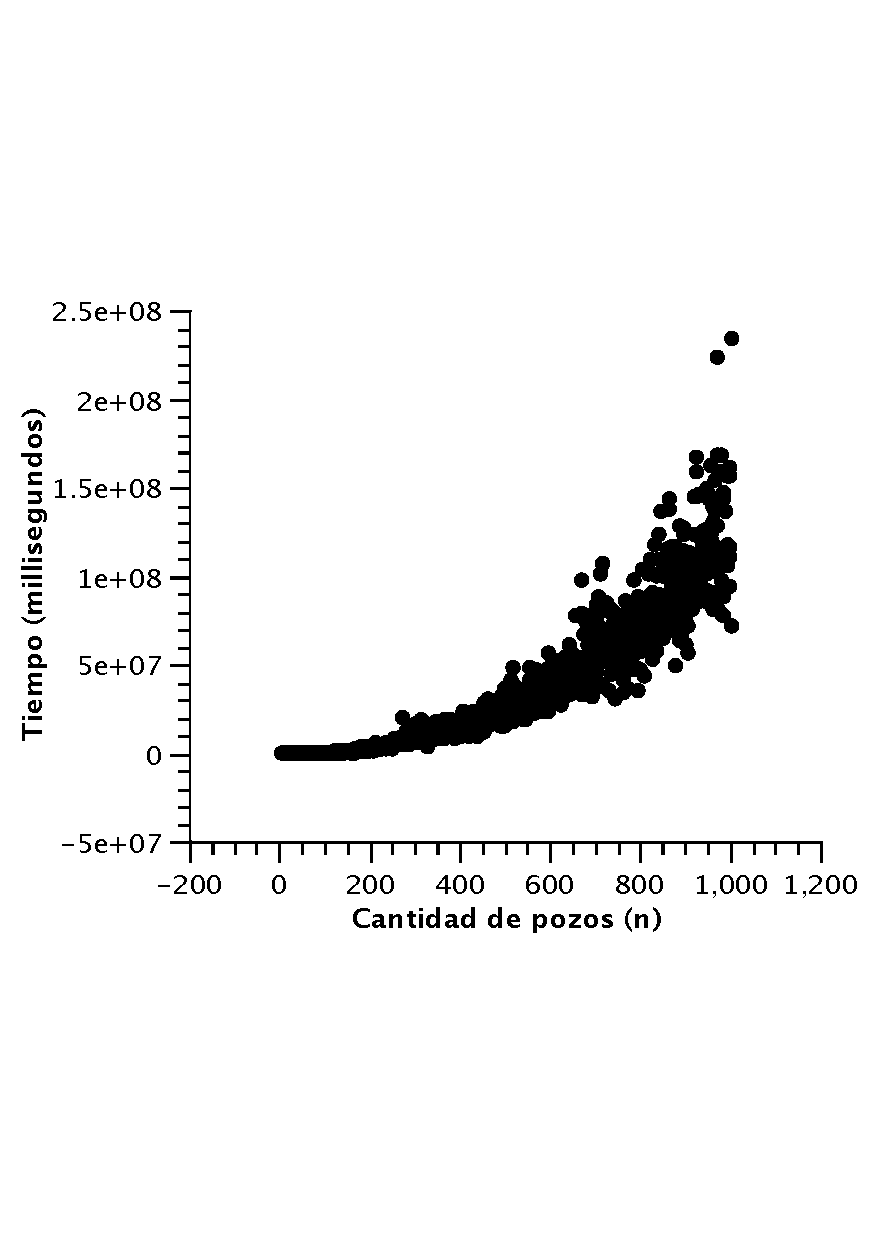
\includegraphics[width=\textwidth]{imagenes/ej3-rawData.pdf}
                \caption*{Tiempos sin procesar, en milisegundos}
        \end{subfigure}%

        \begin{subfigure}[b]{0.5\textwidth}
                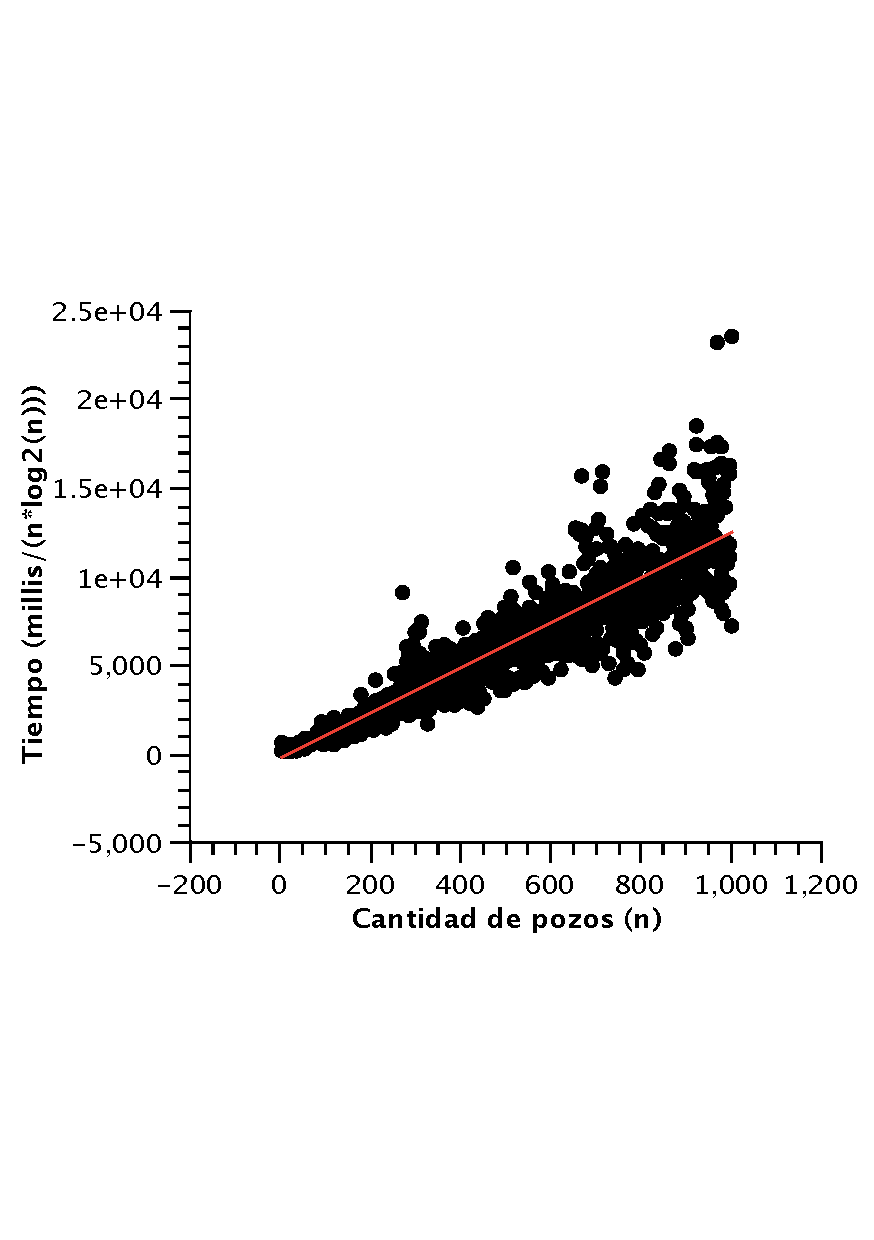
\includegraphics[width=\textwidth]{imagenes/ej3-nlogn.pdf}
                \caption*{Dividiendo a los tiempos por $n \log(n)$}
        \end{subfigure}

\end{figure}

\begin{figure}[H]
        \centering

        \begin{subfigure}[b]{0.5\textwidth}
                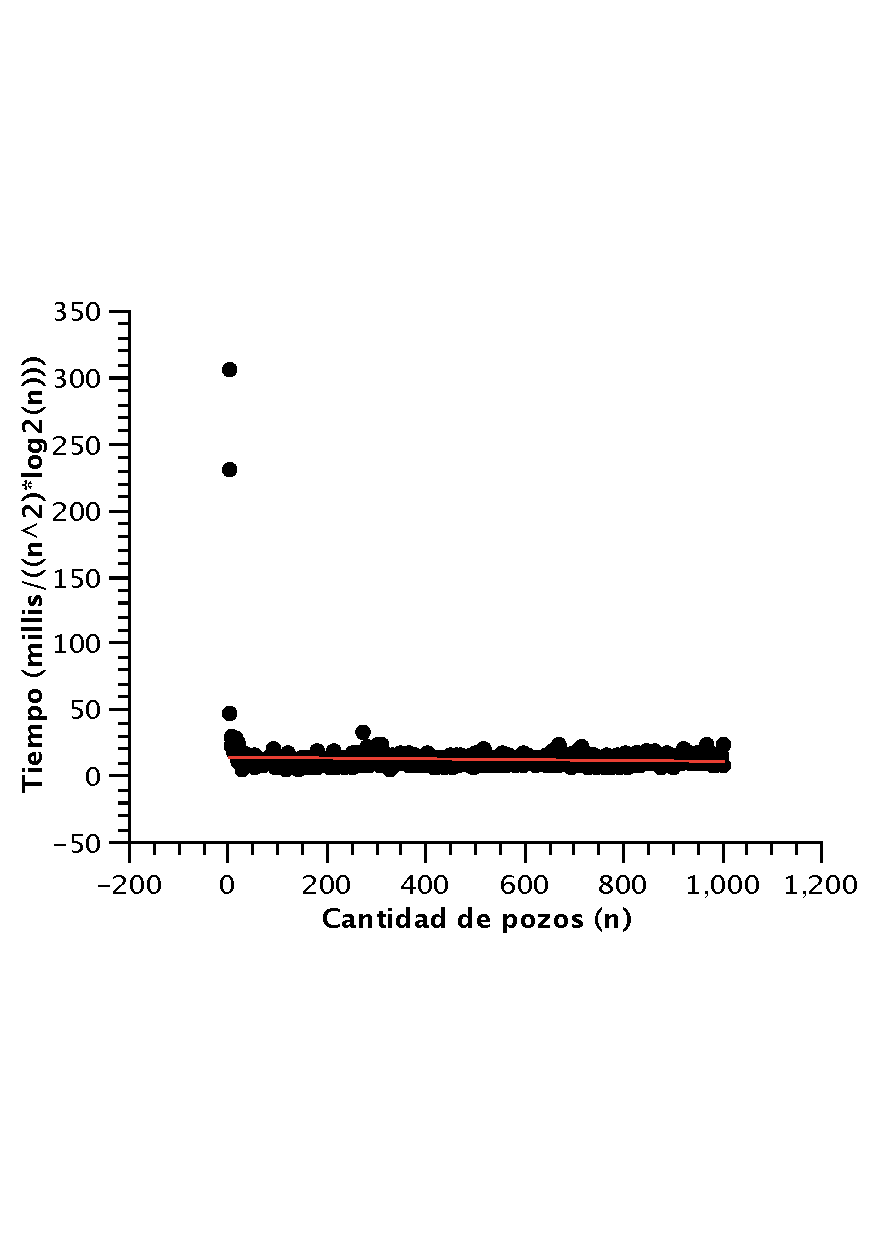
\includegraphics[width=\textwidth]{imagenes/ej3-const.pdf}
                \caption*{Dividiendo a los tiempos por $n^2 \log(n)$}
        \end{subfigure}

\end{figure}


A continuación, adjuntamos una tabla con los últimos 20 valores obtenidos en las instancias aleatorias, teniendo en cuenta que los casos fueron previamente ordenados según el tamaño ($n$):

\begin{table}[H]
\parbox{0.3\textwidth}{
    \begin{tabular}{ | l | l | l | l |}
    \hline
n   &Tiempo(milisegundos) &Tiempo(mili/($n^2 \log(n)$)) &Tiempo(mili/($n \log(n)$)))\\ \hline
980	&106,884,913.7		&11.20017462183745	&10,976.17112940071\\ \hline
981	&148,013,000.5		&15.47597708270933	&15,181.93351813786\\ \hline
982	&143,649,318.15		&14.98692707630785	&14,717.16238893431\\ \hline
983	&88,530,761.25		&9.21626618012942	&9,059.589655067221\\ \hline
984	&77,926,122.55		&8.09462319280639	&7,965.109221721488\\ \hline
985	&96,363,820.55		&9.98806386893941	&9,838.242910905317\\ \hline
986	&137,058,449.3		&14.17515494504867	&13,976.70277581799\\ \hline
987	&109,314,001.3		&11.28115224428363	&11,134.49726510795\\ \hline
988	&116,393,678.25		&11.98570806428229	&11,841.8795675109\\ \hline
989	&95,277,182.2		&9.789957451616216	&9,682.267919648439\\ \hline
990	&106,078,816.3		&10.87624855027109	&10,767.48606476838\\ \hline
991	&156,976,954.55		&16.0600124239817	&15,915.47231216586\\ \hline
992	&112,528,406.3		&11.48768775240836	&11,395.7862503891\\ \hline
993	&117,798,450.6		&11.99972974500853	&11,915.73163679347\\ \hline
994	&109,700,234.25		&11.1506922114351	&11,083.78805816649\\ \hline
995	&156,578,939.15		&15.88147949436476	&15,802.07209689294\\ \hline
996	&117,020,018.95 	&11.84355454694666	&11,796.18032875887\\ \hline
997	&94,736,198.95		&9.567601826537732	&9,538.89902105812\\ \hline
998	&161,853,906.15 	&16.31084667818704	&16,278.22498483067\\ \hline
999	&110,925,527.35		&11.15454731027924	&11,143.39276296896\\ \hline
1,000	&72,523,403.45		&7.27723994203022	&7,277.239942030219\\ \hline
    \end{tabular}
}
\end{table}


Como podemos ver de los gráficos y la tabla suministrada,al dividir los tiempos por $n* \log(n)$, tienden a algo lineal, mientras que al dividir los tiempos por $n^2* \log(n)$, tienden a un número constante. Entonces nuestro algoritmo tendría complejidad $\mathcal{O}(c*n^2* \log(n))$, donde $c$ es la constante a la cual converge el gráfico. Por lo tanto concluimos que los gráficos se condicen con nuestra predicción de complejidad.


\subsubsection{Experimentación con instancias particulares}

Para este problema se nos ocurre probar con instancias de mejor y peor caso.


Una instancia de peor caso sería una donde dado $n$, las tuberías posibles $m$ sean $\frac{n(n-1)}{2}$ y que todas tengan costo menor a $c$, es decir, que dado un pozo, sea posible construir una tubería entre ese pozo y cualquier otro con costo menor al de una refinaría.

El detalle de intervalos es el siguiente:
\begin{itemize}
	\item Cantidad de pozos ($n$): 2 $\leq n \leq$ 1000
    \item Cantidad de tuberías ($m$): $\frac{n(n-1)}{2}$
    \item Costo de refinería ($c$): 1 $\leq c \leq$ 1000
\end{itemize}

No se generaron muestras para n = 1 ya que no hay tuberías posibles.
Generamos 20 instancias aleatorias para cada $n$, variando el $c$ en cada muestra pero fijando para toda tubería un costo de $c-1$ en cada muestra y luego fueron promediadas. Su medición temporal, arroja el siguiente resultado:

\begin{figure}[H]
        \centering
\begin{subfigure}[b]{0.5\textwidth}
                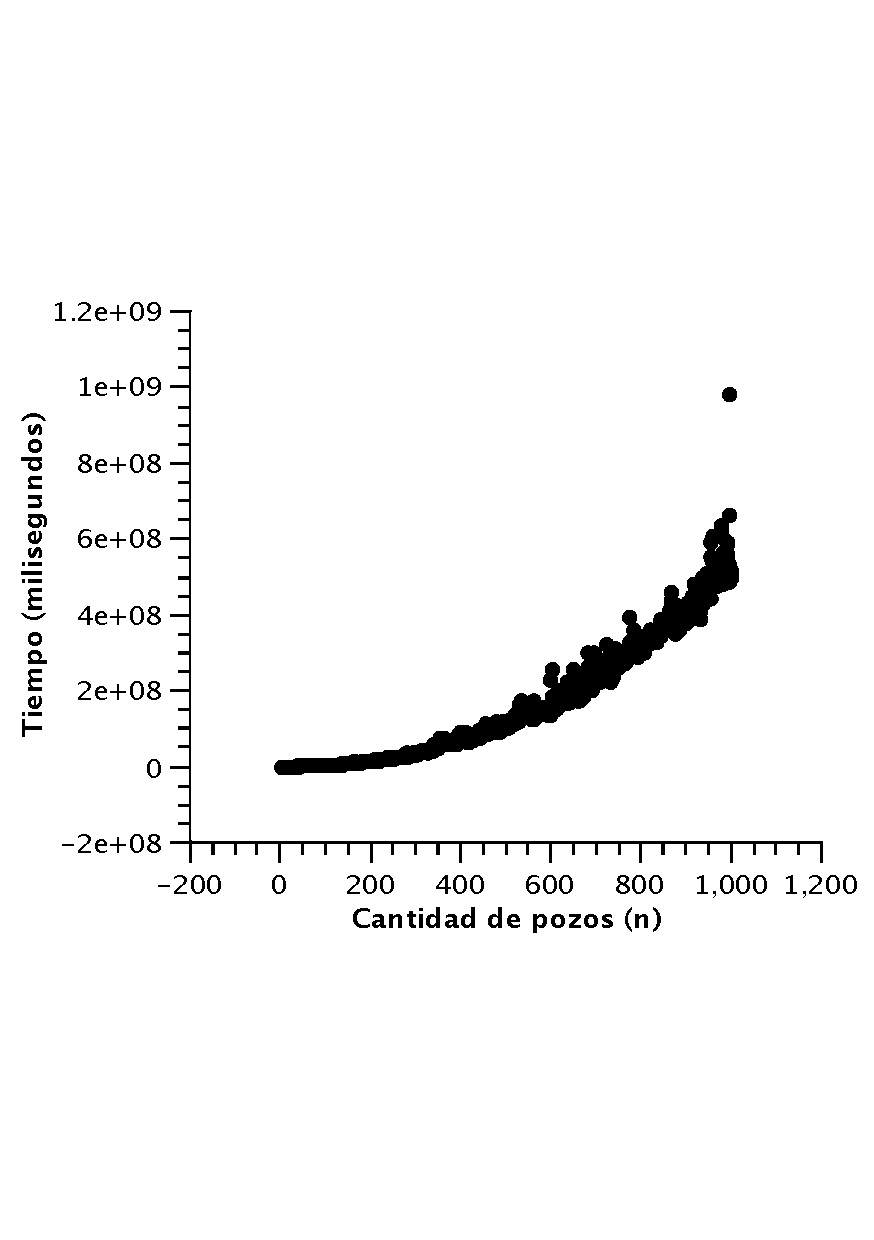
\includegraphics[width=\textwidth]{imagenes/ej3-peor.pdf}
                \caption{Tiempos sin procesar, en milisegundos}
        \end{subfigure}%

        \begin{subfigure}[b]{0.5\textwidth}
                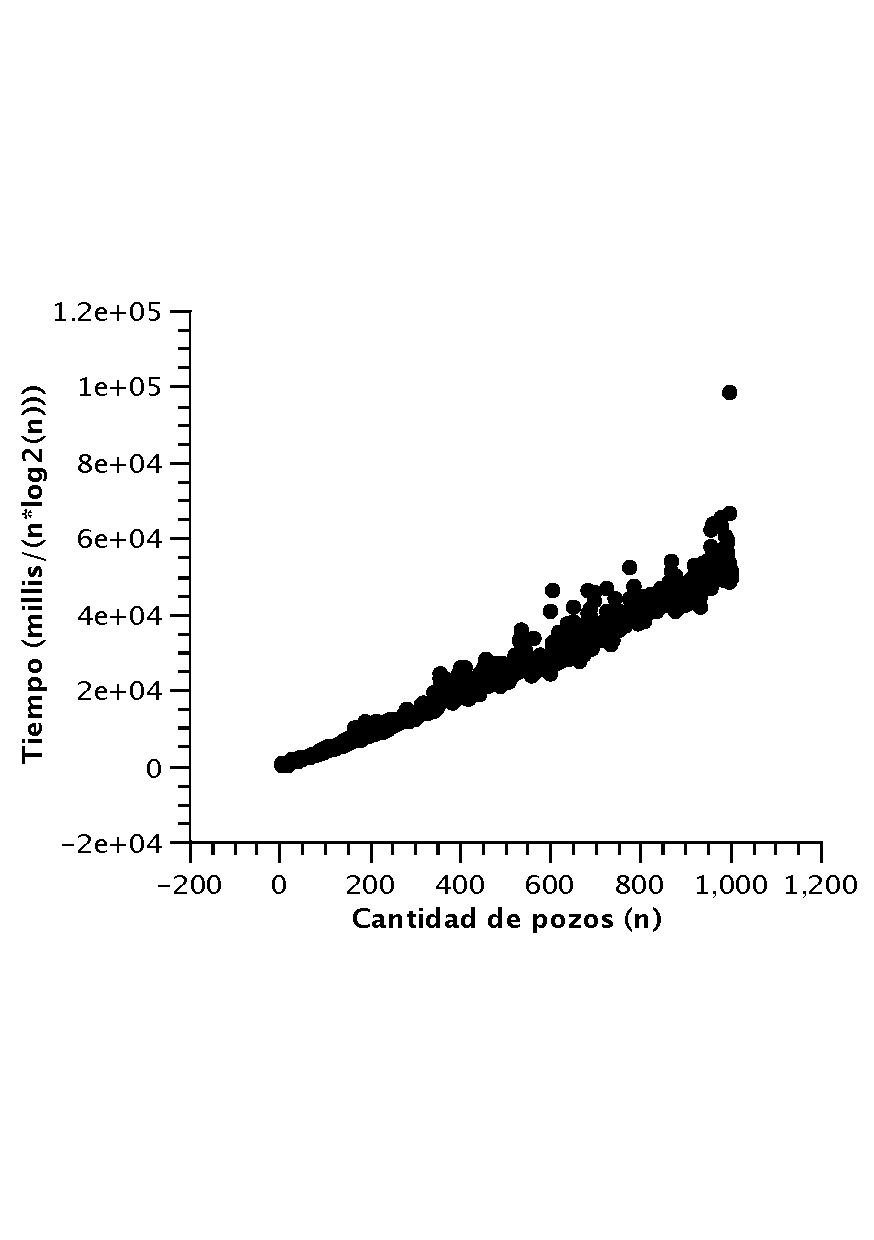
\includegraphics[width=\textwidth]{imagenes/ej3-peor-lineal.pdf}
                \caption{Dividiendo a los tiempos por $n \log(n)$}
        \end{subfigure}

\end{figure}

\begin{figure}[H]
        \centering

        \begin{subfigure}[b]{0.5\textwidth}
                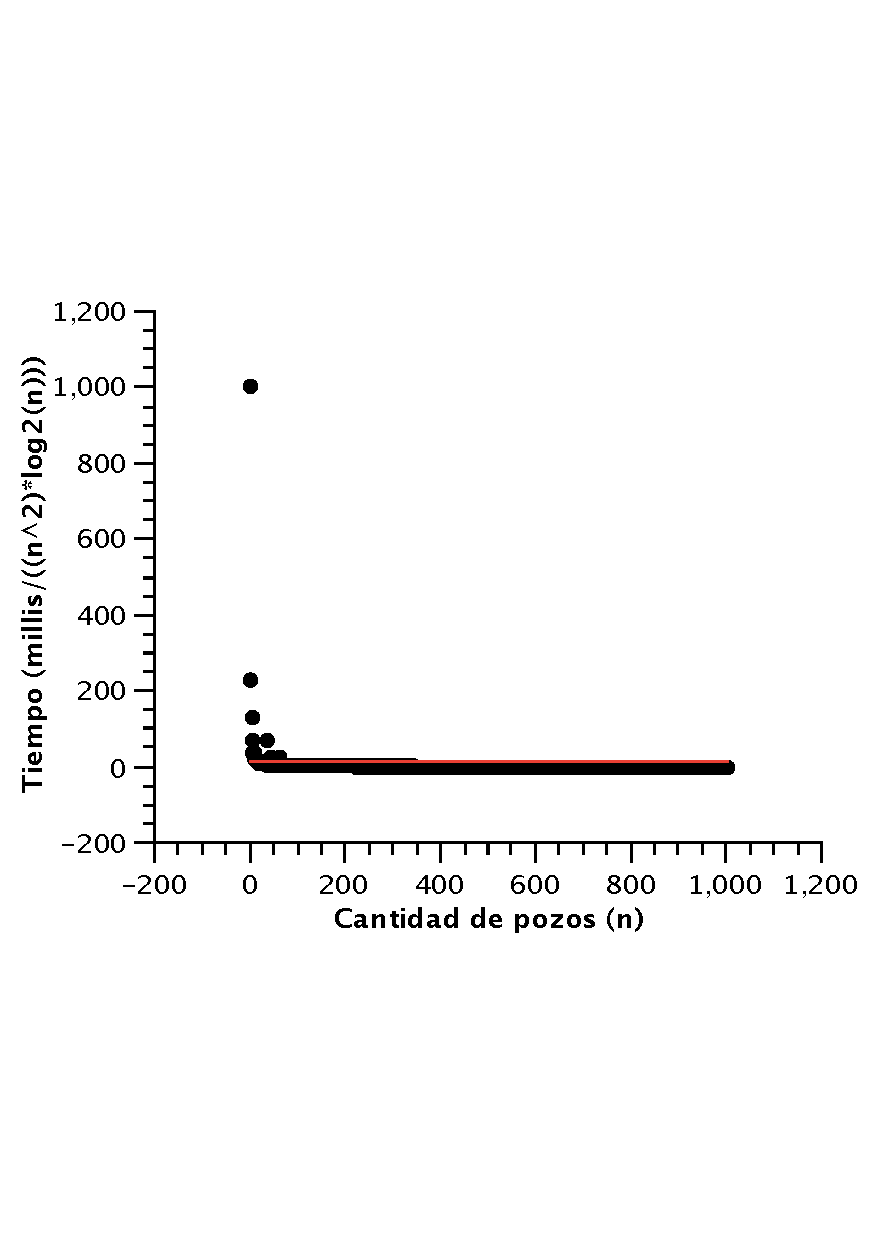
\includegraphics[width=\textwidth]{imagenes/ej3-peor-const.pdf}
                \caption{Dividiendo a los tiempos por $n^2 \log(n)$}
        \end{subfigure}

\end{figure}

A continuación, adjuntamos una tabla con los últimos 20 valores obtenidos en las instancias aleatorias, teniendo en cuenta que los casos fueron previamente ordenados según el tamaño ($n$):

\begin{table}[H]
\parbox{0.3\textwidth}{
    \begin{tabular}{ | l | l | l | l |}
    \hline
n   &Tiempo(milisegundos) &Tiempo(mili/($n^2 \log(n)$)) &Tiempo(mili/($n \log(n)$)))\\ \hline
980	&493,460,879.75	&50,674.23338154993	&0.08452622007433862\\ \hline
981	&482,018,120.4	&49,441.38037692552	&0.09101871660609798\\ \hline
982	&510,165,009.05	&52,267.43419346325	&0.08472145916999867\\ \hline
983	&516,396,402.7	&52,844.22546197011	&0.08947293513434787\\ \hline
984	&561,265,941.75	&57,369.01031618338	&0.07824592057934007\\ \hline
985	&490,971,048.75	&50,125.58045390238	&0.1026006503166199\\ \hline
986	&525,554,033.5	&53,594.01449803058	&0.09532040618344501\\ \hline
987	&570,880,765.55	&58,148.72977958777	&0.1056907440396239\\ \hline
988	&596,367,785.8	&60,674.39059893046	&0.08665430150997189\\ \hline
989	&566,389,457.35	&57,557.68953594214	&0.09656804009648187\\ \hline
990	&508,075,400.3	&51,571.981884774	&0.09234514821696686\\ \hline
991	&583,108,179.7	&59,119.77408159488	&0.1045670681684471\\ \hline
992	&587,978,851.1	&59,544.79875082848	&0.0944663358419995\\ \hline
993	&557,400,980.3	&56,383.08875465296	&0.1324639066988179\\ \hline
994	&590,795,854.55	&59,692.27032416804	&0.07456885483672317\\ \hline
995	&979,012,067	&98,802.68285405725	&0.1032966094149012\\ \hline
996	&662,148,109.4	&66,747.71182669644	&0.09686879345266487\\ \hline
997	&532,542,101.5	&53,621.16473927397	&0.1027177598861123\\ \hline
998	&525,905,149.05	&52,892.15775233119	&0.09732184303195211\\ \hline
999	&486,305,604.75	&48,853.44686677655	&0.1106853151800258\\ \hline
1,000	&497,043,395.25	&49,874.99037230599	&0.08448103791447331\\ \hline
    \end{tabular}
}
\end{table}

Como podemos ver de los gráficos y la tabla suministrada, al dividir los tiempos por $n* \log(n)$, tienden a algo lineal, mientras que al dividir los tiempos por $n^2* \log(n)$, tienden a un número constante. Entonces nuestro algoritmo tendría complejidad $\mathcal{O}(c*n^2* \log(n))$, donde $c$ es la constante a la cual converge el gráfico y esto se cumple incluso en el peor caso. Por lo tanto concluimos que los gráficos se condicen con nuestra predicción de complejidad. \\
\\

Por otro lado, una instancia de mejor caso sería una donde dado $n$, las tuberías posibles $m$ sean una cantidad aleatoria y que todas tengan costo mayor a $c$.

El detalle de intervalos es el siguiente:
\begin{itemize}
	\item Cantidad de pozos ($n$): 2 $\leq n \leq$ 1000
    \item Cantidad de tuberías ($m$): 1 $\leq m \leq \frac{n(n-1)}{2}$
    \item Costo de refinería ($c$): 2 $\leq c \leq$ 1000
\end{itemize}

No se generaron muestras para n = 1 ya que no hay tuberías posibles.
Generamos 20 instancias aleatorias para cada $n$, variando el $c$ en cada muestra pero fijando para toda tubería un costo mayor a $c-1$ en cada muestra y luego fueron promediadas. Su medición temporal, arroja el siguiente resultado:

\begin{figure}[H]
        \centering
\begin{subfigure}[b]{0.5\textwidth}
                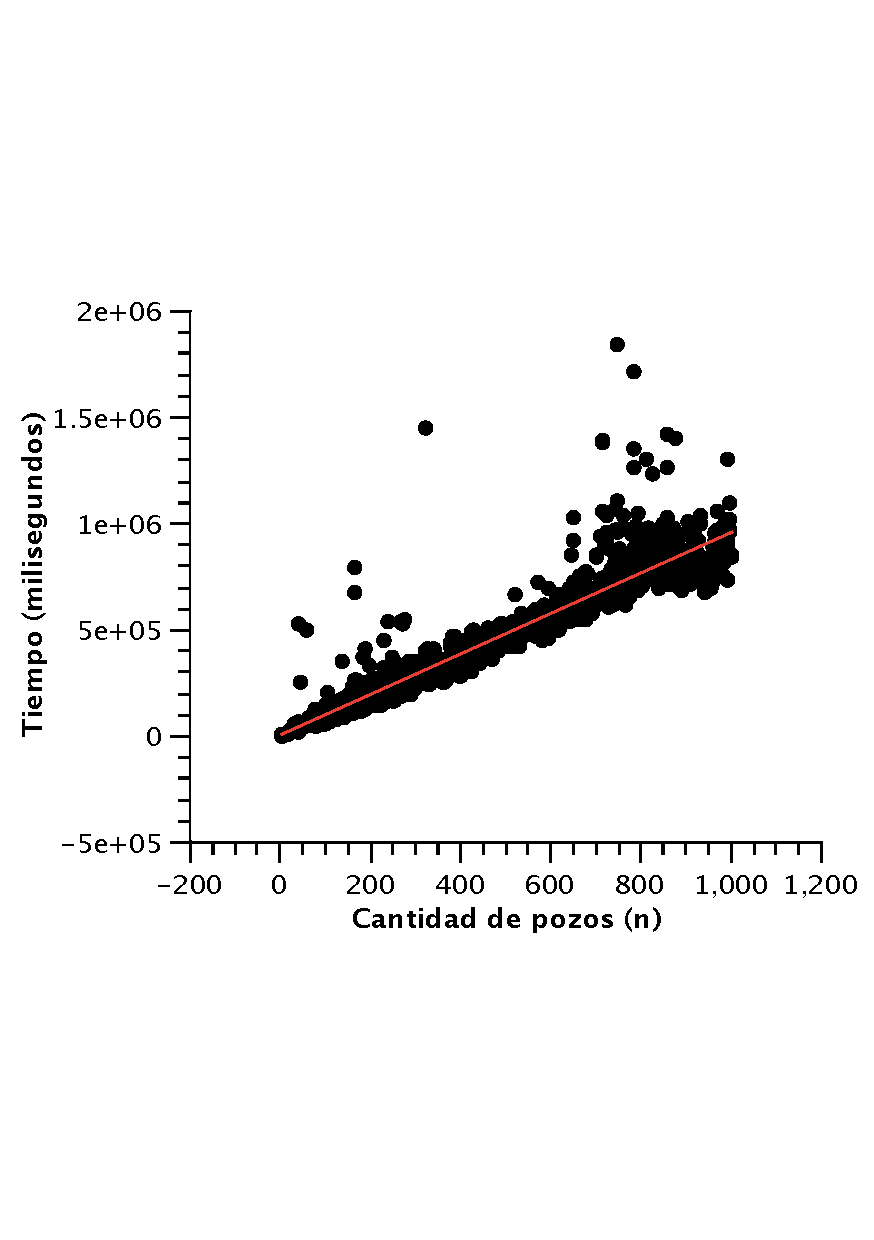
\includegraphics[width=\textwidth]{imagenes/ej3-mejor-lineal.pdf}
                \caption{Tiempos sin procesar, en milisegundos}
        \end{subfigure}%

        \begin{subfigure}[b]{0.5\textwidth}
                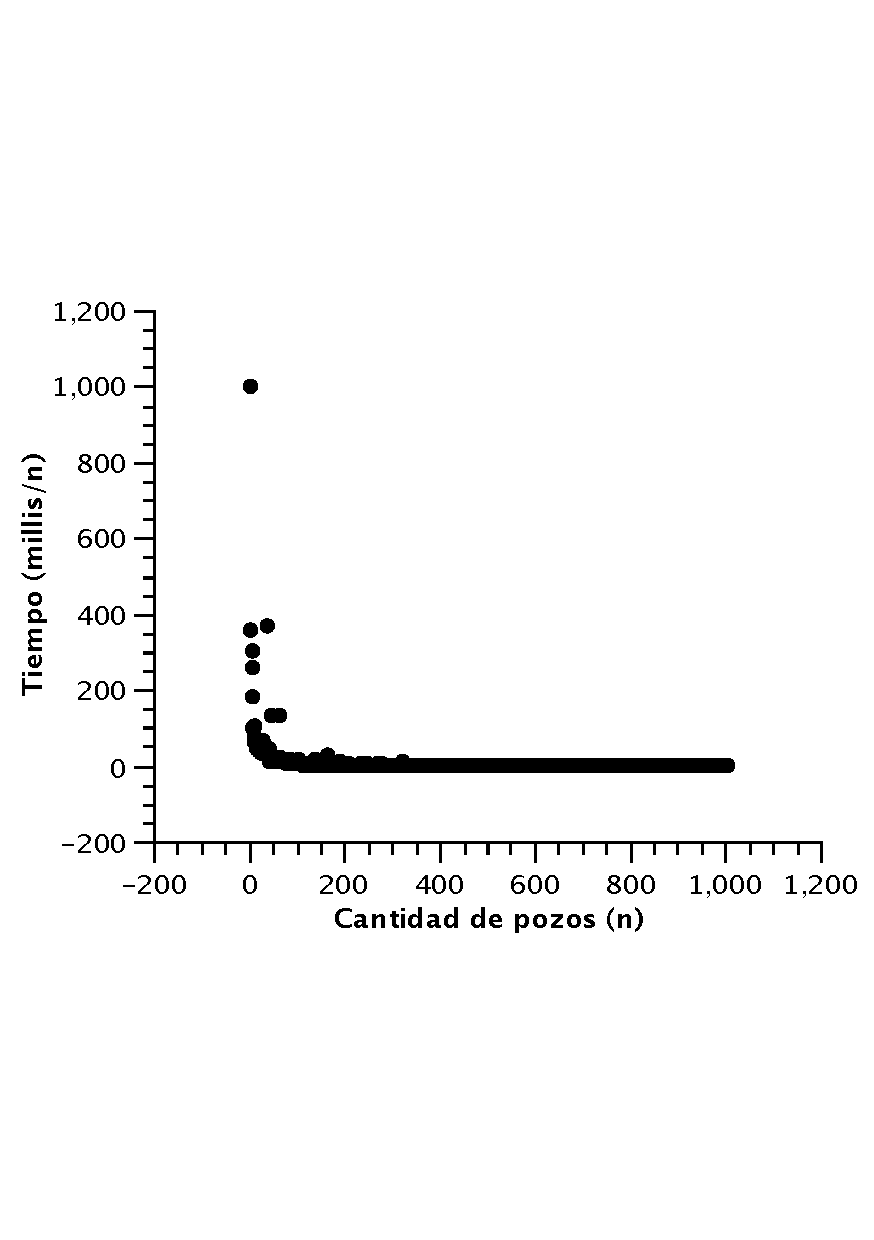
\includegraphics[width=\textwidth]{imagenes/ej3-mejor-const.pdf}
                \caption{Dividiendo a los tiempos por $n$}
        \end{subfigure}

\end{figure}

A continuación, adjuntamos una tabla con los últimos 20 valores obtenidos en las instancias aleatorias, teniendo en cuenta que los casos fueron previamente ordenados según el tamaño ($n$):

\begin{table}[H]
\parbox{0.3\textwidth}{
    \begin{tabular}{ | l | l | l |}
    \hline
n   &Tiempo(milisegundos) &Tiempo(mili/($n)$))\\ \hline
980	&806,646.15	&823.1083163265306\\ \hline
981	&870,507.45	&887.3674311926605\\ \hline
982	&812,053.05	&826.9379327902241\\ \hline
983	&859,470.3	&874.3339776195321\\ \hline
984	&753,265.6	&765.5138211382114\\ \hline
985	&989,880.6	&1,004.954923857868\\ \hline
986	&921,645.45	&934.7316937119675\\ \hline
987	&1,024,139.9	&1,037.629078014184\\ \hline
988	&841,503.3	&851.723987854251\\ \hline
989	&939,813.15	&950.2660768452984\\ \hline
990	&900,665.7	&909.7633333333333\\ \hline
991	&1,022,080.15	&1,031.362411705348\\ \hline
992	&925,351.25	&932.8137600806451\\ \hline
993	&1,300,366.2	&1,309.532930513595\\ \hline
994	&733,606.55	&738.0347585513078\\ \hline
995	&1,018,423.6	&1,023.541306532663\\ \hline
996	&957,110.3	&960.9541164658635\\ \hline
997	&1,017,087.7	&1,020.1481444333\\ \hline
998	&965,732.85	&967.6681863727455\\ \hline
999	&1,100,701.5	&1,101.803303303303\\ \hline
1,000	&841,919.8	&841.9198\\ \hline
1,001	&849,901	&849.0519480519481\\ \hline
\end{tabular}
}
\end{table}

Como podemos ver de los gráficos y la tabla suministrada, al dividir los tiempos por $n$, tienden a un número constante. Entonces nuestro algoritmo tendría complejidad $\mathcal{O}(c*n)$, donde $c$ es la constante a la cual converge el gráfico. Esto sucede porque como todas las tuberías tienen costo mayor a $c$, ninguna es añadida a la cola de prioridad, y por ende no es necesario solucionar el problema ya que la solución de menor costo es poner una refinería en cada pozo. El algoritmo es $\mathcal{O}(n)$ en mejor caso porque es lo que cuesta el ciclo que recorre el UnionFind para ver donde va una refinería, que en este caso es $\mathcal{O}(1)$ porque todas se tienen como raíz a si mismas.

%\newpage
%\appendix
%% \newpage
% \section{Script testing de tiempos Ejercicio 3} \label{sec:script-ej3}
% \lstinputlisting[language=C++]{codigo/timer-test.cpp}

\newpage
\section{Tablas Ejercicio 3} \label{sec:tablas-ej3}

\begin{table}[H]
\parbox{0.3\textwidth}{
  \begin{tabular}{| l | l | l | l |}
    \hline
    $x=n^2-k$ & f(x) & log2(f(x)) & log2(f(x))/x 	\\ \hline
    0	&5,923,061	&22.497912	&inf				\\ \hline
    1	&5,900,691	&22.492453	&22.492453			\\ \hline
    2	&5,959,983	&22.506877	&11.253438			\\ \hline
    3	&5,826,992	&22.474320	&7.491440			\\ \hline
    4	&5,973,392	&22.510119	&5.627530			\\ \hline
    5	&5,857,268	&22.481796	&4.496359			\\ \hline
    6	&5,890,469	&22.489951	&3.748325			\\ \hline
    7	&6,034,068	&22.524699	&3.217814			\\ \hline
    8	&5,934,667	&22.500736	&2.812592			\\ \hline
    9	&6,012,767	&22.519598	&2.502178			\\ \hline
    10	&5,993,751	&22.515028	&2.251503			\\ \hline
    11	&6,021,937	&22.521796	&2.047436			\\ \hline
    12	&6,034,641	&22.524836	&1.877070			\\ \hline
    13	&6,079,293	&22.535472	&1.733498			\\ \hline
    14	&6,160,413	&22.554596	&1.611043			\\ \hline
    15	&6,246,402	&22.574594	&1.504973			\\ \hline
    16	&6,332,631	&22.594374	&1.412148			\\ \hline
    17	&6,439,949	&22.618618	&1.330507			\\ \hline
    18	&6,580,078	&22.649673	&1.258315			\\ \hline
    19	&6,762,607	&22.689148	&1.194166			\\ \hline
    20	&7,056,819	&22.750587	&1.137529			\\ \hline
    21	&7,393,725	&22.817870	&1.086565			\\ \hline
    22	&7,896,252	&22.912737	&1.041488			\\ \hline
    23	&9,165,207	&23.127736	&1.005554			\\ \hline
    24	&11,082,891	&23.401831	&0.975076			\\ \hline
    25	&15,192,578	&23.856863	&0.954275			\\ \hline
%    \textbf{Promedio} & 0,110 & 0,110 & 0,110		\\ \hline
  \end{tabular}
  \caption*{Tabla para $n=5$}
}
\end{table}

\begin{table}[H]
\parbox{0.3\textwidth}{
    \begin{tabular}{| l | l | l | l |}
    \hline
    $x=n^2-k$ & f(x) & log2(f(x)) & log2(f(x))/x 	\\ \hline
    0	&5,565,381	&22.408049	&inf \\ \hline
    1	&5,565,990	&22.408207	&22.408207 \\ \hline
    2	&5,500,844	&22.391221	&11.195611 \\ \hline
    3	&5,548,730	&22.403726	&7.467909 \\ \hline
    4	&5,552,305	&22.404655	&5.601164 \\ \hline
    5	&5,597,932	&22.416462	&4.483292 \\ \hline
    6	&5,616,712	&22.421294	&3.736882 \\ \hline
    7	&5,680,755	&22.437651	&3.205379 \\ \hline
    8	&5,755,858	&22.456600	&2.807075 \\ \hline
    9	&5,852,594	&22.480645	&2.497849 \\ \hline
    10	&5,814,878	&22.471317	&2.247132 \\ \hline
    11	&5,922,181	&22.497697	&2.045245 \\ \hline
    12	&6,270,084	&22.580053	&1.881671 \\ \hline
    13	&6,322,634	&22.592094	&1.737853 \\ \hline
    14	&6,516,583	&22.635684	&1.616835 \\ \hline
    15	&7,002,270	&22.739391	&1.515959 \\ \hline
    16	&7,204,589	&22.780485	&1.423780 \\ \hline
    17	&7,510,993	&22.840572	&1.343563 \\ \hline
    18	&8,480,934	&23.015792	&1.278655 \\ \hline
    19	&8,879,245	&23.082006	&1.214842 \\ \hline
    20	&10,012,036	&23.255232	&1.162762 \\ \hline
    21	&10,944,942	&23.383761	&1.113512 \\ \hline
    22	&12,068,263	&23.524715	&1.069305 \\ \hline
    23	&15,184,908	&23.856135	&1.037223 \\ \hline
    24	&17,689,305	&24.076374	&1.003182 \\ \hline
    25	&21,671,515	&24.369297	&0.974772 \\ \hline
    26	&24,556,881	&24.549624	&0.944216 \\ \hline
    27	&31,239,419	&24.896864	&0.922106 \\ \hline
    28	&43,780,536	&25.383786	&0.906564 \\ \hline
    29	&58,248,061	&25.795707	&0.889507 \\ \hline
    30	&75,611,103	&26.172095	&0.872403 \\ \hline
    31	&96,289,604	&26.520877	&0.855512 \\ \hline
    32	&136,355,286	&27.022795	&0.844462 \\ \hline
    33	&173,505,088	&27.370403	&0.829406 \\ \hline
    34	&244,281,566	&27.863970	&0.819529 \\ \hline
    35	&382,792,021	&28.511986	&0.814628 \\ \hline
    36	&762,531,623	&29.506222	&0.819617 \\ \hline
%    \textbf{Promedio} & 0,110 & 0,110 & 0,110		\\ \hline
  \end{tabular}
  \caption*{Tabla para $n=6$}
}
\end{table}

\begin{table}[H]
\parbox{0.3\textwidth}{
  \begin{tabular}{| l | l | l | l |}
    \hline
    $x=n^2-k$ & f(x) & log2(f(x)) & log2(f(x))/x 	\\ \hline
    0	&5,658,051	&22.431874	&inf \\ \hline
    1	&5,681,202	&22.437765	&22.437765 \\ \hline
    2	&6,076,304	&22.534763	&11.267381 \\ \hline
    3	&6,069,770	&22.533210	&7.511070 \\ \hline
    4	&5,773,935	&22.461123	&5.615281 \\ \hline
    5	&5,758,758	&22.457326	&4.491465 \\ \hline
    6	&5,492,207	&22.388955	&3.731492 \\ \hline
    7	&5,395,753	&22.363393	&3.194770 \\ \hline
    8	&5,551,311	&22.404397	&2.800550 \\ \hline
    9	&5,627,470	&22.424055	&2.491562 \\ \hline
    10	&5,567,587	&22.408621	&2.240862 \\ \hline
    11	&5,766,603	&22.459290	&2.041754 \\ \hline
    12	&5,584,103	&22.412894	&1.867741 \\ \hline
    13	&5,524,277	&22.397354	&1.722873 \\ \hline
    14	&6,066,478	&22.532428	&1.609459 \\ \hline
    15	&5,736,076	&22.451633	&1.496776 \\ \hline
    16	&5,748,738	&22.454814	&1.403426 \\ \hline
    17	&5,602,114	&22.417540	&1.318679 \\ \hline
    18	&5,636,143	&22.426277	&1.245904 \\ \hline
    19	&5,857,809	&22.481930	&1.183259 \\ \hline
    20	&5,757,360	&22.456976	&1.122849 \\ \hline
    21	&6,092,406	&22.538581	&1.073266 \\ \hline
    22	&5,693,843	&22.440971	&1.020044 \\ \hline
    23	&5,645,738	&22.428731	&0.975162 \\ \hline
    24	&5,689,501	&22.439871	&0.934995 \\ \hline
    25	&6,275,472	&22.581292	&0.903252 \\ \hline
    26	&9,863,721	&23.233701	&0.893604 \\ \hline
    27	&9,787,981	&23.222580	&0.860096 \\ \hline
    28	&15,326,389	&23.869514	&0.852483 \\ \hline
    29	&17,433,639	&24.055370	&0.829496 \\ \hline
    30	&46,732,384	&25.477919	&0.849264 \\ \hline
    31	&208,022,561	&27.632165	&0.891360 \\ \hline
    32	&207,625,305	&27.629407	&0.863419 \\ \hline
    33	&248,319,145	&27.887620	&0.845079 \\ \hline
    34	&376,092,555	&28.486513	&0.837839 \\ \hline
    35	&411,197,407	&28.615256	&0.817579 \\ \hline
    36	&448,556,370	&28.740714	&0.798353 \\ \hline
    37	&492,876,908	&28.876652	&0.780450 \\ \hline
    38	&609,898,842	&29.183995	&0.768000 \\ \hline
    39	&1,427,423,303	&30.410766	&0.779763 \\ \hline
    40	&1,758,884,497	&30.712014	&0.767800 \\ \hline
    41	&2,463,547,271	&31.198090	&0.760929 \\ \hline
    42	&2,262,938,362	&31.075550	&0.739894 \\ \hline
    43	&3,067,540,200	&31.514435	&0.732894 \\ \hline
    44	&8,222,938,242	&32.937007	&0.748568 \\ \hline
    45	&9,802,502,055	&33.190503	&0.737567 \\ \hline
    46	&7,629,766,484	&32.828992	&0.713674 \\ \hline
    47	&11,287,976,621	&33.394068	&0.710512 \\ \hline
    48	&11,509,510,828	&33.422107	&0.696294 \\ \hline
    49	&20,280,864,861	&34.239400	&0.698763 \\ \hline
%    \textbf{Promedio} & 0,110 & 0,110 & 0,110	\\ \hline
  \end{tabular}
  \caption*{Tabla para $n=7$}
}
\end{table}

\begin{table}[H]
\parbox{0.3\textwidth}{
  \begin{tabular}{| l | l | l | l |}
    \hline
    $x=n$ & f(x) & log2(f(x)) & log2(f(x))/(x*x) 	\\ \hline
    1	&6,894,821	&22.717082	&22.7171 			\\ \hline
    2	&7,258,736	&22.791287	&5.69782 			\\ \hline
    3	&8,437,732	&23.008424	&2.55649 			\\ \hline
    4	&9,649,562	&23.202032	&1.45013 			\\ \hline
    5	&20,032,573	&24.255844	&0.970234 			\\ \hline
    6	&696,757,144	&29.376081	&0.816002 		\\ \hline
    7	&20,679,794,169	&34.267503	&0.699337 		\\ \hline
    8	&299,907,350,785	&38.125726	&0.595714 	\\ \hline
%    \textbf{Promedio} & 0,110 & 0,110 & 0,110		\\ \hline
  \end{tabular}
  \caption*{Tabla para $k=0$}
}
\end{table}

 \begin{table}[H]
 \parbox{0.7\textwidth}{
\begin{tabular}{ |l|l|l|l|l|l|l| }
  \hline
  k & \multicolumn{2}{|c|}{$n=3$} & \multicolumn{2}{|c|}{$n=4$} & \multicolumn{2}{|c|}{$n=5$} \\ \hline
  {}& con podas& sin podas&	con podas&	sin podas&	con podas&	sin podas \\ \hline
  0&	5,599,710&	5,421,781&	5,473,768&	5,784,018&	5,605,871&	6,544,455 \\ \hline
  1&	5,612,436&	5,604,190&	5,510,945&	5,947,644&	5,536,143&	7,107,637 \\ \hline
  2&	5,450,933&	5,936,583&	5,521,407&	6,005,466&	5,495,775&	8,050,800 \\ \hline
  3&	5,487,297&	5,705,466&	5,477,040&	6,037,971&	5,589,136&	9,446,413 \\ \hline
  4&	5,617,896&	5,717,293&	5,509,341&	6,381,715&	5,553,264&	9,799,520 \\ \hline
  5&	5,431,101&	5,728,081&	5,555,143&	6,812,464&	5,518,550&	11,924,701 \\ \hline
  6&	5,471,542&	5,566,319&	5,506,907&	7,172,540&	5,596,573&	14,523,360 \\ \hline
  7&	5,672,431&	5,727,042&	5,533,490&	8,411,726&	5,486,095&	27,464,034 \\ \hline
  8&	5,467,644&	5,688,279&	5,514,259&	11,391,268&	5,541,097&	39,776,822 \\ \hline
  9&	7,611,266&	8,436,007&	5,544,664&	13,931,410&	5,584,355&	66,818,916 \\ \hline
  10&			{}&			{}&	5,565,962&	18,574,226&	5,509,177&	64,198,701 \\ \hline
  11&			{}&			{}&	5,529,941&	24,196,471&	5,548,982&	100,469,504 \\ \hline
  12&			{}&			{}&	5,564,854&	30,429,761&	5,589,544&	176,433,434 \\ \hline
  13&			{}&			{}&	5,551,530&	37,589,963&	5,615,420&	242,246,035 \\ \hline
  14&			{}&			{}&	5,578,268&	48,436,269&	5,628,109&	377,537,126 \\ \hline
  15&			{}&			{}&	5,522,458&	58,712,605&	5,659,103&	683,836,846 \\ \hline
  16&			{}&			{}&	6,956,095&	86,716,207&	5,767,523&	893,203,595 \\ \hline
  17&			{}&			{}&			{}&			{}&	5,788,079&	1,326,734,757 \\ \hline
  18&			{}&			{}&			{}&			{}&	5,974,659&	2,031,435,579 \\ \hline
  19&			{}&			{}&			{}&			{}&	6,048,999&	3,165,594,743 \\ \hline
  20&			{}&			{}&			{}&			{}&	6,283,413&	3,781,117,314 \\ \hline
  21&			{}&			{}&			{}&			{}&	6,259,904&	5,603,863,234 \\ \hline
  22&			{}&			{}&			{}&			{}&	6,193,765&	9,993,456,118 \\ \hline
  23&			{}&			{}&			{}&			{}&	6,006,958&	14,970,489,604 \\ \hline
  24&			{}&			{}&			{}&			{}&	5,502,917&	18,238,644,771 \\ \hline
  25&			{}&			{}&			{}&			{}&	8,168,827&	32,265,934,044 \\ \hline
\end{tabular}
 \caption*{Tabla para $n=3,\ 4\ y\ 5$ comparando con Podas vs. sin Podas}
}
\end{table}

\end{document}